\documentclass{book}
\usepackage{titling}
\usepackage{multirow}
\usepackage{setspace}
\usepackage{makeidx}
\usepackage{tikz}
\usepackage{subfigure}
\usepackage{braket}
\usepackage{graphicx}
\usepackage{array}

\usepackage{qcircuit}
\usepackage{graphicx}

\usepackage{tabularray}
\usepackage{amsmath}
\usepackage{circuitikz}
\usepackage{amssymb}
\usepackage{setspace}
\usepackage{amsmath}
\usepackage{xepersian}
\settextfont{XB Zar}
\linespread{1.5}



\makeatletter
\def\TikzBipolePath#1#2{\pgf@circ@bipole@path{#1}{#2}}
\def\CircDirection{\pgf@circ@direction}
\makeatother

% TikZ libraries `calc` needed now to tweak bracket.
\usetikzlibrary{backgrounds,fit,decorations.pathreplacing,calc}

\begin{document}
\tableofcontents
\section{مقدمه}	
در عصر حاضر بواسطه‌ی رشد و توسعه‌ی نظریه‌ی اطلاعات کوانتومی و سرمایه‌گذاری های مالی و انسانی بسیار در این زمینه،‌شاهد افزایش تعداد علاقمندان به این حوزه هستیم. در این پا .....

\chapter{آشنایی با مفاهیم اولیه}
\section{کیوبیت}

یک کیوبیت\footnote{\lr{Qubit}}، معادل یک واحد اطلاعات کوانتومی می‌باشد. این مفهوم معادل مفهوم کلاسیک بیت\footnote{\lr{Binary Bit}} می‌باشد. به طور کلی هر کیوبیت حاوی دو بیت اطلاعات است. برای تبیین یک کیوبیت از خصوصیات سامانه های کوانتومی، بهره‌می‌بریم. کیوبیت یک سیستم کوانتومی با فضای دوبعدی است. برای تعیین این دوبعد می‌توان ا ز یکی از خصویات سامانه های کوانتومی استفاده کرد. 

برخلاف بیت ها که مقادیر ثابت 0 یا 1 را به خود می‌گیرند؛ یک کیوبیت می‌تواند در یک حالت «برهمنهی کوانتومی» باشد؛ این بدان معناست که یک کیوبیت بواسطه‌ی مشاهده ناظر به یکی از حالات 0 یا یک تبدیل شود. این مهم‌ترین مزیت استفاده از کیوبیت‌هاست. بیان ریاضی یک کیوبیت ،در حالت برهمنهی، به شرح زیر است:
\vspace{2cm}
$$
\left\{
\begin{array}{ll}
	  \vert \psi \rangle = \alpha\vert 0 \rangle + \beta\vert 1 \rangle \\
	  \alpha^2 + \beta^2 = 1
\end{array}
\right.
$$
\vspace{2cm}

\newpage
کت‌های $\vert 0 \rangle$ و $\vert 1 \rangle$ بیانگر پایه‌های فضای 
محاسباتی\footnote{\lr{Computational Basis Vectors}} هستند؛ و مقادیر $\alpha^2$ و $\beta^2$ بیانگر احتمال وقوع هر یک از این حالات، در صورت مشاهده، می‌باشند. نمایش بردار $\psi$ به شرح زیر است:
\begin{center}
\begin{tikzpicture}
	
	% Define the axes
	\draw[->] (-2,0)--(2,0) node[right]{$\vert 0 \rangle$};
	\draw[->] (0,-2)--(0,2) node[above]{$\vert 1 \rangle$};
	
	% Draw the vector
	\draw[black,-stealth] (0,0)--(1,2) node[anchor=south west]{$\vec{\psi}$};
	
	% Label the components of the vector
	\node[below] at (1,0) {$$};
	\node[left] at (0,2) {$$};
	
\end{tikzpicture}
\end{center}

در بسیاری از مواقع برای سهولت در محاسبات، عملگر‌ها و حالات کوانتومی به کمک ماتریس‌ها نمایش داده ‌می‌شوند. فرم ماتریسی هر یک از حالات ذکر شده در بالا به شرح زیر است:

\begin{equation}
	\vert 1 \rangle = \begin{pmatrix} 0 \\ 1 \end{pmatrix}
	\hspace{2cm}
	\vert 0 \rangle = \begin{pmatrix} 1 \\ 0 \end{pmatrix}	
\end{equation}

برای تعریف کیوبیت ها، راه های زیادی وجود دارد، حالات قطبش فوتون،‌اسپین الکترون،‌یا سطوح انرژی اتم،‌هریک می‌توانند تعیین کننده‌ی بردار‌های فضای کیوبیت باشند.

\section{bloch vector - computayional basis - fourier basis-comp vs superpos basis}

Chapter 1 chuang book

Consider the circuit shown in Figure 1.17, which applies Uf to an input not in the
computational basis. Instead, the data register is prepared in the superposition (|0〉 +
|1〉)/√2, which can be created with a Hadamard gate acting on |0〉. Then we apply Uf ,
resulting in the state:
% https://g.co/bard/share/2972a6a63b24

\newpage
\section{گیت‌های کوانتومی}
گیت‌های کوانتومی\footnote{\lr{Quantum Gates}} یکی از اولین و مهم‌ترین اجزای‌ مدار‌های کوانتومی ‌می‌باشند. این گیت‌ها عملگر‌هایی با قابلیت اثر‌گذاری روی کیوبیت‌ها می‌باشند. با اعمال یک گیت کوانتومی بر روی یک یا چند کیوبیت، می‌توان تغییرات مدنظر خود را روی کیوبیت اعمال کرد. با کمک این گیت‌ها می‌توان باعث برهم‌نهی کوانتومی یا رمز‌گذاری داده در داخل یک یا چند کیوبیت شد.

\subsection{انواع گیت کوانتومی}
گیت‌های کوانتومی، دارای انواع مختلف گوناگونی می‌باشند. به طور کلی گیت‌های کوانتومی، عملگر‌هایی یکه و بازگشت‌پذیر می‌باشند. 
\subsection*{گیت هادامارد}
مهم‌ترین گیت کوانتومی،‌گیت هادامارد\footnote{\lr{Hadamard gate}} است. با اعمال اثر این گیت روی یک کیوبیت، آن کیوبیت به‌یک حالت برهم نهی‌ کوانتومی‌ گذار‌ می‌کند. به عبارت دیگر هر یک از زیرحالات این حالت برهم‌نهی، با احتمال یکسانی قابل رخ دادن‌ هستند. 
\vspace{1cm}
$$
H\ket{0} = \frac{1}{\sqrt{2}} (\ket{0} + \ket{1})
\hspace{2cm}
H\ket{1} = \frac{1}{\sqrt{2}} (\ket{0} - \ket{1})
$$
\vspace{1cm}

این گیت کوانتومی‌ به صورت خطی روی یک دسته‌ کت اثر مي‌کند. نمایش ماتریسی این گیت‌کوانتومی به شرح زیر است:
\begin{center}
	\[
	H = \frac{1}{\sqrt{2}}
	\begin{pmatrix}
		1 & 1 \\
		1 & -1
	\end{pmatrix}
	\]
\end{center}





\begin{align*}
	H |0\rangle = l\frac{1}{\sqrt{2}} \begin{pmatrix} 1 & 1 \\ 1 & -1 \end{pmatrix} \begin{pmatrix} 1 \\ 0 \end{pmatrix} \
	= \frac{1}{\sqrt{2}} \begin{pmatrix} 1 \\ 1 \end{pmatrix} \
	= \frac{1}{\sqrt{2}} (|0\rangle + |1\rangle)
\end{align*}

\begin{align*}
	H |1\rangle = l\frac{1}{\sqrt{2}} \begin{pmatrix} 1 & 1 \\ 1 & -1 \end{pmatrix} \begin{pmatrix} 0 \\ 1 \end{pmatrix} \
	= \frac{1}{\sqrt{2}} \begin{pmatrix} 1 \\ -1 \end{pmatrix} \
	= \frac{1}{\sqrt{2}} (|0\rangle - |1\rangle)
\end{align*}

این گیت کوانتومی، یک گیت بازگشت‌پذیر است؛ یعنی اگر این گیت روی یک حالت کوانتومی اثر کند؛‌ می‌تواند آن را از حالت برهمنهی خارج کند. 

برای اعمال این گیت کوانتومی، فقط به یک کیوبیت نیاز داریم. به اصطلاح این گیت،‌
یک \lr{Single-Qubit Quantum gate} می‌باشد.

نمایش این گیت‌کوانتومی در مدار با علامت زیر است:
\Qcircuit @C=1em @R=1.2em {
	& & \qw & \gate{H} & \qw \\
	& & & & \\
}


\subsection*{گیت CNOT}
% https://www.youtube.com/watch?v=0ECbWBBbglw
% https://www.youtube.com/watch?v=emHhNFf5AVM

گیت کوانتومی \lr{CNOT}\footnote{ controlled-NOT gate or controlled-X gate}، به عنوان گیت منطقی نیز یاد می‌شود. این گیت کوانتومی معادل گیت \lr{NOT} کلاسیک می‌باشد.
به‌طور معمول، برای اعمال اثر این گیت کوانتومی نیاز به دو کیوبیت داریم. این گیت کوانتومی فقط و فقط در مواقعی که «کیوبیت کنترل\footnote{Controled Qubit}» دارای مقدار $\vert 1 \rangle$ باشد، باعث تغییر وضعیت «کیوبیت هدف\footnote{Target Qubit}» می‌شود.\\

کیوبیت کنترلی: کیوبیتی است که عملکرد کیوبیت دیگری به نام کیوبیت هدف را کنترل می کند. کیوبیت کنترل تعیین می کند که آیا کیوبیت هدف برگردانده شود یا خیر. اگر کیوبیت کنترل در حالت |0⟩ باشد، کیوبیت هدف بدون تغییر باقی می‌ماند. اگر کیوبیت کنترل در حالت |1⟩ باشد، کیوبیت هدف برگردانده می شود.\\

کیوبیت هدف: همان کیوبیتی است که توسط کیوبیت کنترل بر روی آن عمل می شود. بسته به وضعیت کیوبیت کنترل، کیوبیت هدف را می توان برگرداند یا بی‌تغییر رها کند.\\



خلاصه‌ای از عملکرد این عملگر به شرح زیر است:\\
\textbf{ببین چرا از این نماد به جای تنسور پراداکت استفاده شده}
\begin{latin}
\begin{tabular}{ccccc}
	&&&&\\
	|A & B$\rangle$ &	&  |A &B $\oplus$ A $\rangle$  \\
	|control$\rangle$ & |target$\rangle$ & Effect CNOT Gate &|control$\rangle$ & |target$\rangle$ \\
	------- & -------- & -------- & -------- & --------  \\
	|0$\rangle$ & |0$\rangle$ & $\Longrightarrow$ &|0$\rangle$ & |0$\rangle$ \\
	|0$\rangle$ & |1$\rangle$ & $\Longrightarrow$ &|0$\rangle$ & |1$\rangle$ \\
	|1$\rangle$ & |0$\rangle$ & $\Longrightarrow$ &|1$\rangle$ & |1$\rangle$ \\
	|1$\rangle$ & |1$\rangle$ & $\Longrightarrow$ &|1$\rangle$ & |0$\rangle$
\end{tabular}
\end{latin}


نمایش ماتریسی این گیت کوانتومی به شکل زیر است:
\begin{figure}[ht]
	\centering
	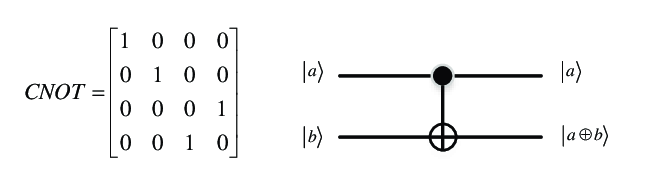
\includegraphics[width=\linewidth]{Matrix-representation-and-quantum-circuit-of-CNOT-gate.png}
	\caption{نمایش ماتریسی و نمایش گیت کوانتومی \lr{CNOT}}
	\label{CNOT}
\end{figure}


در شکل بالا گیت \lr{CNOT} در مدار کوانتومی به تصویر درآمده است. کیوبیت کنترل شده  حالت $\vert a \rangle$ و کیوبیت هدف حالت $\vert b \rangle$ می‌باشد.


با اعمال این عملگر به حالت $\vert 10\rangle$ داریم:
$$
\text{CNOT} \ket{1} = \begin{pmatrix}
	1 & 0 & 0 & 0 \\
	0 & 1 & 0 & 0 \\
	0 & 0 & 0 & 1 \\
	0 & 0 & 1 & 0
\end{pmatrix} \begin{pmatrix}
	1 \\
	0 \\
	0 \\
	0
\end{pmatrix} = \begin{pmatrix}
	0 \\
	0 \\
	0 \\
	1
\end{pmatrix} = \ket{1}
$$


$$
\text{CNOT} \ket{11} = \begin{pmatrix}
	1 & 0 & 0 & 0 \\
	0 & 1 & 0 & 0 \\
	0 & 0 & 0 & 1 \\
	0 & 0 & 1 & 0
\end{pmatrix} \begin{pmatrix}
	1 \\
	1 \\
	0 \\
	0
\end{pmatrix} = \begin{pmatrix}
	0 \\
	1 \\
	0 \\
	0
\end{pmatrix} = \ket{10}
$$
\vspace{2cm}


از این گیت کوانتومی‌، برای بسیاری مدار‌ها و شبیه‌سازی‌های کوانتومی، از جمله تلپورت، درهمتنیدگی و ...،استفاده می‌شود.





\subsubsection*{گیت توفولی}
گیت کوانتومی توفولی،‌یک نوع خاص از گیت \lr{CNOT} است. سازوکار این گیت مشابه گیت \lr{CNOT} می‌‌باشد؛‌ با این تفاوت که با در نظر گرفتن وضعیت دو کیوبیت کنترل شده، وضعیت کیوبیت سوم را تغییر می‌دهد. خلاصه ای از عملکرد این گیت کوانتومی به شرح زیراست:

به بیان دیگر اگر دو کیوبیت کنترل شده،‌ مقدار یک داشته باشند؛‌ کیوبیت هدف مقدارش تغییر می‌کند.
فرم ماتریسی این عملگر به شکل زیر است:

این گیت کوانتومی در مدار کوانتومی به شکل زیر نشان داده می‌شود:

\subsection*{گیت تغییر فاز}
گیت تغییر فاز\footnote{Phase shift gate}، یکی از گیت های مهم کوانتومی‌ می‌باشد. این گیت با ضرب کردن یک عدد ثابت در فاز یک کیوبیت، باعث تغییر فاز کیوبیت می‌شود. این گیت کوانتومی در بسیاری از الگوریتم‌های سرچ کوانتومی به‌کار می‌رود. این گیت بدین صورت تعریف می‌شود:

فرم ماتریسی این گیت به شرح زیر است:

این گیت کوانتومی در مدار کوانتومی به شکل زیر نشان داده می‌شود:

\subsection*{گیت دوران}
گیت دوران، \footnote{Rotation gate}، باعث دوران حالت کیوبیت، در فضای هیلبرت ‌می‌شود. پایه‌های فضای هیلبرت مذکور بردار های................................... هستند. نمایش این گیت کوانتومی به شرح زیر است:

فرم ماتریسی این گیت به شرح زیر است:
نمایش این گیت در مدار کوانتومی به شرح زیراست:


\subsection{Swap gate}

% https://www.youtube.com/watch?v=_p7i2v21Ys8&t=188s
% https://www.youtube.com/watch?v=F2okky5vD8k&list=PL1826E60FD05B44E4&index=11



\section{مدار‌های کوانتومی}
مدار‌های ‌کوانتومی\footnote{quantum circuit}، یک دسته از گیت ها‌ی کوانتومی،که با یک توالی بخصوص قرار گرفته اند، ‌می‌باشند. این کیوبیت ها، با توالی یاد شده، روی یک یا چند دسته کیوبیت، اثر داده ‌می‌شوند. 

مدار‌های کوانتومی، یکی از اولین مفهوم‌های بکار‌رفته برای تعریف کامپیوتر‌های کوانتومی‌ می‌باشند. برای تعریف و شبیه‌سازی هریک از پدیده‌ها و الگوریتم‌های کوانتومی، نیاز به پیاده‌سازی یک مدار به‌خصوص داریم.


مدارهای کوانتومی یک ابزار قدرتمند برای محاسبات کوانتومی هستند. آنها می توانند برای پیاده سازی طیف گسترده ای از الگوریتم های کوانتومی، از جمله الگوریتم شاور برای رمزگشایی اعداد صحیح و الگوریتم گروور برای جستجوی پایگاه داده های بدون ترتیب استفاده شوند.

\subsubsection{شباهت ها و تفاوت های مدارهای کلاسیک و کوانتومی}
مدارهای کوانتومی مشابه مدارهای کلاسیک هستند، اما از دروازه های کوانتومی به جای دروازه های منطقی کلاسیک استفاده می کنند. دروازه های کوانتومی عملیات قابل برگشت هستند که می توانند برای دستکاری حالت کوانتومی یک کوبیت استفاده شوند.

\textbf{شباهت ها}

\begin{itemize}
	\item هر دو مدار کوانتومی و کلاسیک از یک دنباله عملیاتی تشکیل شده اند که به یک مجموعه داده اعمال می شوند.
	\item هر دو مدار را می توان به صورت گرافیکی با نماد مشابهی نشان داد.
	\item هر دو مدار می توانند برای پیاده سازی الگوریتم ها استفاده شوند.
\end{itemize}

\textbf{تفاوت ها}

\begin{itemize}
	\item مدارهای کوانتومی از کیوبیت ها، که معادل کوانتومی مفهوم بیت هستند، به عنوان واحد پایه داده خود استفاده می کنند. 
	\item مدارهای کلاسیک از بیت ها ، که بیت های کلاسیک هستند ، به عنوان واحد پایه داده خود استفاده می کنند.
	\item مدارهای کوانتومی از دروازه های کوانتومی ، که عملیات قابل برگشت هستند ، به عنوان عملیات پایه خود استفاده می کنند.
	\item  مدارهای کلاسیک از دروازه های منطقی ، که عملیات برگشت ناپذیر هستند ، به عنوان عملیات پایه خود استفاده می کنند.
	\item مدارهای کوانتومی می توانند خواص مکانیک کوانتوم را ، مانند برهمنهی و درهمتنیدگی ، برای انجام کارهایی که برای رایانه های کلاسیک غیرممکن است ، بهره مند شوند.
\end{itemize}



\begin{table}[ht]
	\centering
	\begin{tabular}{|p{100pt}|p{100pt}|p{100pt}|}
		\hline
		ویژگی & مدار کوانتومی &مدار کلاسیک \\
		\hline
		واحد پایه داده & کیوبیت & بیت \\
		\hline
	      عملیات پایه & دروازه های کوانتومی & دروازه های منطقی \\
		\hline
		برگشت پذیری & قابل برگشت & برگشت ناپذیر \\
		\hline
	\end{tabular}
	\caption{This is a table with 3 rows and 3 columns.}
\end{table}



\subsubsection{اجزای مدار‌های کوانتومی و سایز آن }
\paragraph{اندازه مدار کوانتومی}

اندازه یک مدار کوانتومی تعداد دروازه های موجود در مدار است. پیچیدگی یک الگوریتم کوانتومی اغلب با اندازه مدار کوانتومی مورد نیاز برای پیاده سازی آن اندازه گیری می شود.


\paragraph{کوبیت}

کوبیت ها واحد پایه اطلاعات در محاسبات کوانتومی هستند. آنها می توانند در یک superposition از دو حالت ، 0 و 1 باشند. این بدان معنی است که یک کوبیت می تواند هم 0 و هم 1 باشد ، که یک ویژگی به نام superposition کوانتومی است. کوبیت ها همچنین می توانند به هم متصل شوند ، که به این معنی است که حالت یک کوبیت به حالت کوبیت دیگر وابسته است.
\paragraph{دروازه}
دروازه ها عملیاتی هستند که روی کوبیت ها اعمال می شوند. آنها می توانند برای ایجاد superpositions ، انجام چرخش ها و درهم تنیدگی کوبیت ها استفاده شوند. انواع مختلفی از دروازه ها وجود دارد ، اما برخی از رایج ترین آنها شامل دروازه Hadamard ، دروازه CNOT و دروازه Toffoli است.

\paragraph{عملیات}

عملیات اقداماتی هستند که روی کوبیت ها انجام می شوند. آنها می توانند اندازه گیری ها ، راه اندازی ها یا سایر اقدامات باشند. اندازه گیری ها برای فروپاشی حالت کوانتومی یک کوبیت به یک مقدار قطعی ، 0 یا 1 استفاده می شود. راه اندازی ها برای تنظیم حالت یک کوبیت به یک مقدار خاص ، 0 یا 1 استفاده می شوند.




اجزای اساسی یک مدار کوانتومی کوبیت ها ، دروازه ها و عملیات هستند. این اجزا برای ایجاد الگوریتم های کوانتومی استفاده می شوند که الگوریتم هایی هستند که فقط می توانند روی یک رایانه کوانتومی اجرا شوند. مدارهای کوانتومی یک ابزار قدرتمند برای محاسبات کوانتومی هستند و پتانسیل انقلابی در بسیاری از زمینه های مختلف ، از جمله رمزنگاری ، شیمی و یادگیری ماشین را دارند.

\subsection{نحوه‌ی نمایش مدار‌های کوانتومی}


مدارهای کوانتومی با استفاده از نماد گرافیکی مشابه نمودارهای مدار استفاده شده در محاسبات کلاسیک نوشته می شوند. محور افقی یک مدار کوانتومی زمان را نشان می دهد و محور عمودی کوبیت ها را نشان می دهد. دروازه ها توسط جعبه ها نشان داده می شوند و خطوط بین جعبه ها نشان دهنده ارتباطات بین کوبیت ها است.

\newpage
\chapter{برنامه‌نویسی کوانتومی}
برنامه نویسی کوانتومی فرآیند طراحی و پیاده‌سازی دنباله هایی از دستورالعمل هایی موسوم مدارهای کوانتومی می‌باشد، با استفاده از گیت ها، سوئیچ ها و عملگرها برای دستکاری وضعیت کوانتومی یک کیوبیت به پردازش مسائل می‌پردازیم.

مدارهای کوانتومی یک نمایش گرافیکی از الگوریتم های کوانتومی هستند، این الگوریتم هایی فقط روی یک کامپیوتر کوانتومی قابل اجرا هستند.

برنامه نویسی کوانتومی یک زمینه نسبتاً جدید است و تعدادی زبان برنامه نویسی کوانتومی مختلف در دسترس است. برخی از محبوب ترین زبان های برنامه نویسی کوانتومی عبارتند از Qiskit، Cirq و Quil.

برنامه نویسی کوانتومی یک زمینه پیچیده و چالش برانگیز است، اما این پتانسیل را دارد که در بسیاری از زمینه های مختلف از جمله رمزنگاری، شیمی و یادگیری ماشین انقلابی ایجاد کند. با قدرتمندتر شدن کامپیوترهای کوانتومی، برنامه نویسی کوانتومی اهمیت فزاینده ای پیدا خواهد کرد.
\section{تفاوت کامپیوتر کلاسیک و کوانتومی}

**کامپیوترهای کوانتومی در مقابل کامپیوترهای کلاسیک**

کامپیوترهای کوانتومی و کامپیوترهای کلاسیک دو نوع بسیار متفاوت از رایانه هستند. کامپیوترهای کوانتومی از بیت‌های کوانتومی (کوبیت‌ها) برای ذخیره اطلاعات استفاده می‌کنند، در حالی که کامپیوترهای کلاسیک از بیت‌ها استفاده می‌کنند. کوبیت‌ها می‌توانند در حالت برهم‌نهی دو حالت، 0 و 1، به‌طور همزمان باشند، در حالی که بیت‌ها فقط می‌توانند در یک حالت به‌طور همزمان باشند. این تفاوت در نحوه ذخیره اطلاعات امکان محاسباتی را برای کامپیوترهای کوانتومی فراهم می‌کند که برای کامپیوترهای کلاسیک غیرممکن است.

علاوه بر تفاوت در نحوه ذخیره اطلاعات، کامپیوترهای کوانتومی و کلاسیک در نحوه انجام محاسبات نیز متفاوت هستند. کامپیوترهای کوانتومی از مکانیک کوانتوم برای انجام محاسبات استفاده می‌کنند، در حالی که کامپیوترهای کلاسیک از منطق بولی استفاده می‌کنند. این تفاوت در نحوه انجام محاسبات نیز به کامپیوترهای کوانتومی امکان می‌دهد تا برای برخی از وظایف، محاسباتی را بسیار سریع‌تر از کامپیوترهای کلاسیک انجام دهند.

کاربردهای بالقوه کامپیوترهای کوانتومی بسیار گسترده است. آنها می‌توانند برای رمزگشایی روش‌های رمزنگاری فعلی، شبیه‌سازی مولکول‌ها و آموزش مدل‌های یادگیری ماشینی که بسیار دقیق‌تر از مدل‌های فعلی هستند، استفاده شوند. کامپیوترهای کوانتومی هنوز در مراحل اولیه توسعه هستند، اما پتانسیل تغییر جهان را دارند. هنگامی که کامپیوترهای کوانتومی قدرتمندتر شوند، قادر به حل مشکلاتی خواهند بود که برای کامپیوترهای کلاسیک در حال حاضر غیرممکن است.

 برخی از مثال‌های خاص از نحوه استفاده از کامپیوترهای کوانتومی:

* رمزنگاری: کامپیوترهای کوانتومی می‌توانند برای رمزگشایی روش‌های رمزنگاری فعلی استفاده شوند، که تأثیر عمده‌ای بر امنیت آنلاین خواهد داشت.
* شیمی: کامپیوترهای کوانتومی می‌توانند برای شبیه‌سازی مولکول‌ها استفاده شوند، که می‌تواند به دانشمندان در توسعه داروها و مواد جدید کمک کند.
* یادگیری ماشینی: کامپیوترهای کوانتومی می‌توانند برای آموزش مدل‌های یادگیری ماشینی که بسیار دقیق‌تر از مدل‌های فعلی هستند، استفاده شوند.

آینده محاسبات کوانتومی بسیار روشن است. هنگامی که کامپیوترهای کوانتومی قدرتمندتر شوند، قادر به حل مشکلاتی خواهند بود که برای کامپیوترهای کلاسیک در حال حاضر غیرممکن است. این می‌تواند منجر به پیشرفت‌های عمده در بسیاری از زمینه‌های مختلف شود.
\section{comp vs simulation}
% computer vs simulator https://www.youtube.com/watch?v=2qcvgXaDdfU
% https://www.youtube.com/watch?v=0RPFWZj7Jm0	

بسیاری از مسائل کوانتومی و بسیاری از الگوریتم‌های کوانتومی قابل شبیه‌سازی روی کامپیوتر‌های کوانتومی می‌باشند. بنابرین یک سوال به‌واقع مهم مطرح می‌شود: \textbf{چرا به یک کامپیوتر کوانتومی نیاز داریم؟}

در هنگام محاسبات کوانتومی،‌ کامپیوتر‌های کلاسیک دارای محدودیت‌هایی هستند. به طور مشابه کامپیوتر‌های کوانتومی نیز دارای معایبی هستند؛ که قابل بحث و بررسی هستند. دراین بخش به این مزایا و معایب هرکدام از کامپیوترها می‌پردازیم و در ادامه به اهداف تعریف شده برای کامپیوترهای کوانتومی می‌پردازیم.


\subsection{تفاوت کامپیوترهای کوانتومی و شبیه‌سازهای کلاسیک}
همانطور که در بخش‌های قبلی گفته شد؛ کامپیوترهای کوانتومی با استفاده از کیوبیت‌ها تعریف می‌شوند. یک کیوبیت به صورت یک ترکیب خطی از حالت $\vert0\rangle$ و $\vert1\rangle$ تعریف می‌شود:

\begin{center}
	$\vert\psi\rangle = \alpha\vert0\rangle + \beta\vert1\rangle$
\end{center}

هریک از حالات داخل رابطه‌ی بالا به صورت یک ماتریس قابل تعریف هستند. به طور مشابه هریک از عملگر های کوانتمی را می‌توان به صورت یک ماتریس تعریف کرد. ماتریس‌هایی مشابه ماتریس پائولی یا در مقیاس‌های بالاتر ماتریس فردکین که برای سه کیوبیت تعریف می‌شود؛ و محاسبات را سریع می‌سازد.



از طرفی دیگر تعداد محاسبات در مدار‌های کلاسیک به تعداد حالات مسأله بستگی دارد. در محاسبات کلاسیک هرچه تعداد حالات بالاتر برود؛ پیچیدگی محاسبات بالاتر‌می‌رود و حتی اغلب با حالت نمایی رشد می‌کنند. این درحالیست که در محاسبات کوانتومی هر یک حالات مختلف مسأله به یک دنیای موازی کوانتومی شیفت داده می‌شود و از این طریق محاسبات به زمان و منابع کمتری نیاز دارد.


مهم‌ترین عامل در سطح پیچیدگی محاسبات کوانتومی همدوسی می‌باشد. 
🤖 : درکودانس در محاسبات کوانتومی مهم است زیرا اصلی ترین منبع خطا در این سیستم ها است. کوبیت ها، واحد های اصلی اطلاعات در محاسبات کوانتومی، بسیار حساس به محیط خود هستند و می توانند به راحتی توسط  interactions با فوتون ها، الکترون ها و سایر ذرات دکور شوند. این می تواند باعث شود که کوبیت ها خواص کوانتومی خود را مانند superposition و entanglement که برای انجام محاسبات کوانتومی ضروری هستند، از دست بدهند.

Decoherence می تواند توسط عوامل مختلفی ایجاد شود، از جمله:

* **دما:** کوبیت ها در دماهای بالاتر مستعد دکوراسیون هستند. این به این دلیل است که هرچه دما بالاتر باشد، کوبیت ها انرژی بیشتری دارند و بیشتر احتمال دارد با محیط خود تعامل داشته باشند.
* **تکان ها:** کوبیت ها همچنین می توانند توسط ارتعاشات دکور شوند. این به این دلیل است که ارتعاشات می توانند باعث حرکت کوبیت ها شوند، که می تواند حالت های کوانتومی آنها را مختل کند.
* **تابش الکترومغناطیسی:** کوبیت ها می توانند توسط تابش الکترومغناطیسی، مانند نور و امواج رادیویی، دکور شوند. این به این دلیل است که تابش الکترومغناطیسی می تواند با الکترون های کوبیت ها تعامل داشته باشد و باعث از دست رفتن خواص کوانتومی آنها شود.

Decoherence یک مانع بزرگ برای توسعه ابررایانه های کوانتومی است. برای ساخت یک رایانه کوانتومی عملی، باید راه هایی برای کاهش دکوراسیون پیدا کرد. این یک مشکل دشوار است، اما تعدادی از مسیرهای تحقیقاتی امیدوار کننده وجود دارد، مانند:

* **کوبیت ها را تا دماهای بسیار پایین سرد کنید:** این می تواند انرژی کوبیت ها را کاهش دهد و آنها را کمتر مستعد تعامل با محیط خود کند.
* **استفاده از مواد با زمان های coherence طولانی:** برخی از مواد، مانند ابررساناها، زمان های coherence بسیار طولانی دارند که آنها را برای استفاده در رایانه های کوانتومی بسیار مناسب می کند.
* **توسعه الگوریتم های جدید تصحیح خطا کوانتومی:** الگوریتم های تصحیح خطا کوانتومی می توانند برای تشخیص و تصحیح خطاهایی که توسط decoherence ایجاد می شوند استفاده شوند.

Decoherence یک مشکل پیچیده و چالش برانگیز است، اما یکی از مهمترین مشکلاتی است که در حال حاضر توسعه رایانه های کوانتومی را پیش رو دارد. با ادامه تحقیقات، به احتمال زیاد قادر خواهیم بود دکوراسیون را برطرف کنیم و رایانه های کوانتومی عملی بسازیم که می توانند مشکلاتی را حل کنند که برای رایانه های کلاسیک غیرقابل حل هستند.

+++++++

در شبیه‌سازی با کامپیوترکلاسیک نمی‌توان میزان ناهمدوسی را شبیه سازی کرد. 
عکس از چنل یوتیب بذار و کدها رو باهم مقایسه کن.

\newpage


\section{IBM Quantum computer and Qiskit}
\newpage



\chapter{الگوریتم‌های‌کوانتومی‌}


چه گونه‌ای از مسائل محاسباتی قابل اجرا با مدارهای کوانتومی می‌باشند؟ 
تفاوت و برتری مدار‌های کوانتومی نسبت به مدار‌های کلاسیک چیست؟
آیا می‌توان یک حوزه‌ی خاص را تعیین کرد؛ به گونه‌ای که عملکرد کامپیوترهای‌‌کوانتومی نسبت به کامپیوتر‌های کلاسیک مزیت داشته باشند؟

در این بخش می‌خواهیم به طور خلاصه این سوالات را پاسخ دهیم و توضیح دهیم چگونه می‌توان از کامپیوتر‌های کوانتومی به شکلی سودمند استفاده کنیم.

\section{موازی سازی کوانتومی}

موازی‌سازی کوانتومی\footnote{Quantum parallelism}، پایه‌واساس بسیاری از الگوریتم‌های کوانتومی است. با گذار یک حالت کوانتومی به حالت برهمنهی کوانتومی، درحین محاسبات کوانتومی یک تابع نظیر \lr{f(x)}، می‌تواند مقادیر مختلف \lr{x} را به طور همزمان بررسی کند. این درحالیست که در محاسبات کلاسیک به دلیل ماهیت بیت‌های اطلاعات، تابع \lr{f(x)} فقط می‌تواند یکی از مقادیر مجاز برای \lr{x} را بررسی کند.


فرض کنید تابع f ،یک تابع تک-کیوبیت، به صورت زیر تعریف شده است:\\
\begin{center}
	$f (x) : \{0, 1\} \rightarrow \{0, 1\}$\\
\end{center}

روش مناسب برای محاسبه این تابع در یک کامپیوتر کوانتومی، با در نظر گرفتن دو کیوبیت که در حالت $\vert x, y\rangle$شروع می شود. با یک توالی مناسب از گیت های منطقی می توان این حالت را به $\vert f(x) \oplus x, y\rangle$ تبدیل کرد که در آن $\oplus$ بیانگر جمع مدوله با پایه‌2 می‌باشد.

\footnote{Modulo 2 is a mathematical operation that returns the remainder of a division by 2. For example, 5 mod 2 is 1, because 5 divided by 2 has a quotient of 2 and a remainder of 1.
	
	The symbol "⊕" is often used to indicate addition modulo 2. So, the expression "5 ⊕ 3" would be evaluated as follows:
	
	5 ⊕ 3 = (5 + 3) mod 2 = 8 mod 2 = 0
	This is because 8 divided by 2 has a quotient of 4 and a remainder of 0.
	
	Modulo 2 is a useful operation in many different areas of mathematics, including cryptography, computer science, and number theory. It is also used in everyday life, for example, when checking whether a number is even or odd.
	
	Here are some other examples of modulo 2:
	
	1 mod 2 = 1
	2 mod 2 = 0
	3 mod 2 = 1
	4 mod 2 = 0
	5 mod 2 = 1}

هریک از دسته‌های کیوبیت، \textbf{رجیستر کوانتومی} نامیده‌می‌شوند. اولین رجیستر، «رجیستر داده» و دومین رجیستر «رجیستر هدف» نامیده می‌شود.\\
ازین پس در این بخش به عامل گذار $\vert x, y \rangle \rightarrow \vert x, y \oplus f(x) \rangle$، عنوان «تابع \lr{$U_{f}$}» را اطلاق خواهیم کرد. لازم به ذکرست که این تبدیل، یک تبدیل یکه به شمار می‌آید.\footnote{اثبات این مطلب از حوصله‌ی بحث خارج است.}


اگر \lr{y = 0} آنگاه مقدار دومین کیوبیت بعد از اعمال تابع \lr{$U_{f}$} برابر با مقدار \lr{f(x)} خواهد بود.

 \begin{center}
 	 \begin{figure}[ht]
 		\centering
 		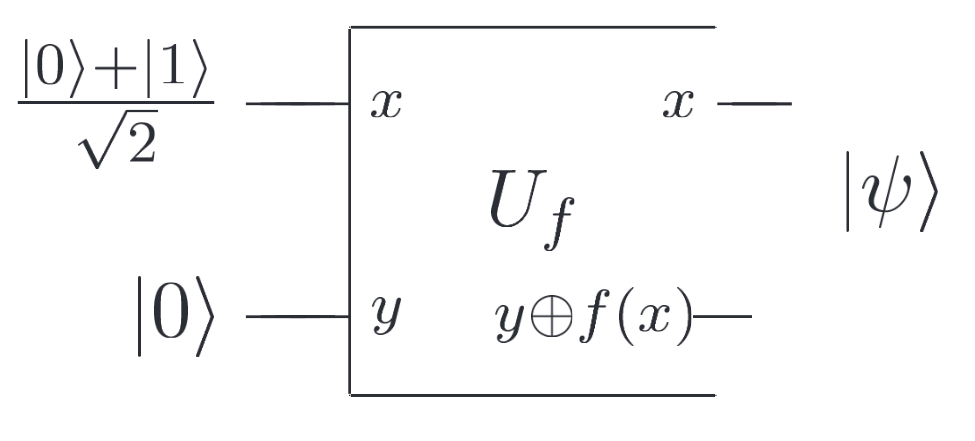
\includegraphics[width=0.8\textwidth]{Uforacle.png}
 		\caption{مدار کوانتومی برای ارزیابی $f (0)$ و $f (1)$ به طور همزمان. Uf مدار کوانتومی است که ورودی هایی مانند $\vert x, y\rangle$ را به $\vert x, y \rangle \rightarrow \vert x, y \oplus f(x) \rangle$، تصویر می‌کند.}
 	\end{figure}
 \end{center}

در شکل بالا مقادیر ورودی داده شده به تابع \lr{$U_{f}$} در پایه‌های محاسباتی قرار ندارند. رجیستر داده در حالت برهمنهی  قرار دارد. این حالت برهمنهی را می‌توان با اعمال گیت هادامارد بر حالت کوانتومی $\vert 0 \rangle$ ایجاد کرد. پس از ایجاد این حالت، تابع \lr{$U_{f}$} را به حالت جدید اعمال می‌کنیم:
\begin{center}
	$\frac{\vert 0,f(0) \rangle +\vert 1,f(1) \rangle }{\sqrt{2}}$
\end{center}

این یک حالت استثنایی است! جملات مختلف کسر بالا حاوی اطلاعاتی در مورد f (0) وf (1) می‌باشند؛ به‌نحوی که انگار f (x) را برای دو مقدار x به طور همزمان ارزیابی کرده ایم، این ویژگی به "موازی  سازی کوانتومی" موسوم می‌باشد. بر خلاف موازی سازی کلاسیک، که در آن هر یک مدارهای متعددی دارند ساخته شده برای محاسبه f (x) به طور همزمان اجرا می شوند، در اینجا برای ارزیابی تابع برای چندین مقدار x به طور همزمان، یک مدار f (x) (با قابلیت برهمنهی کوانتومی)استفاده می شود.

این فرآیند را می توان به راحتی  با استفاده از یک عمل کلی به نام تبدیل هادامارد، به توابعی با تعداد بیت دلخواه تعمیم داد. این عمل فقط تعداد n گیت هادامارد است که به طور موازی روی n کوبیت عمل می کنند.

برای مثال در شکل زیر؛ دو کیوبیت در حالت $\vert 0 \rangle$ آماده شده‌‌اند. پس از اعمال گیت‌های هادامارد بر روی این رجیستر به خروجی زیر خواهیم رسید: 

\begin{center}
	$ \Biggl( \frac{\vert 0 \rangle + \vert 1 \rangle}{\sqrt{2}}\Biggl)\Biggl( \frac{\vert 0 \rangle + \vert 1 \rangle}{\sqrt{2}}\Biggl) = \frac{\textbar00\rangle + \textbar01\rangle + \textbar10\rangle + \textbar11\rangle}{\sqrt{2}}$

\end{center}

از نماد $\operatorname{H} \otimes 2$ به عنوان نشانه‌ی عملکرد موازی دو گیت هادامارد استفاده می‌کنیم؛از علامت $\otimes$ به عنوان تانسور یاد می‌کنیم. به طور کلی نتایج اعمال موازی گیت هادامارد روی \lr{n} کیوبیت روی حالت کوانتومی برابرست با:

\begin{center}
	\[\frac{1}{\sqrt{2}} \sum_{x} \vert x \rangle\]
\end{center}


در اینجا، $\sum$ نشان دهنده جمع بر روی همه مقادیر ممکن \lr{x} است، و ما$\operatorname{H} \otimes n$  را برای نشان دادن این عمل می نویسیم.
اعمال تبدیل هادامارد روی یک بهمنهی کوانتومی برابر از همه حالت های محاسباتی تولید می کند؛ و با استفاده از فقط $n$ گیت، یک برهمنهی از $2n$ حالت تولید می کند.
\begin{center}
	\begin{figure}[ht]
		\centering
		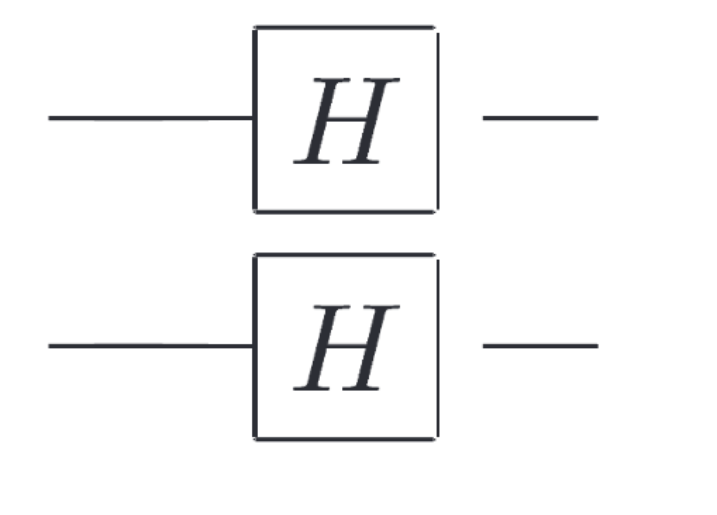
\includegraphics[width=0.8\textwidth]{Multyhadamard.png}
		\caption{اعمال تبدیل هادامارد $\operatorname{H} \otimes n$روی دو کیوبیت}
	\end{figure}
\end{center}

تبدیل هادامارد $\operatorname{H} \otimes 2$ روی دو بیت کوانتومی پیاده می‌شود. ارزیابی موازی کوانتومی یک تابع f(x) با ورودی n بیتی x و خروجی 1 بیتی، به روش زیر قابل پیاده‌سازی می‌باشد:

\begin{enumerate}
	\item ابتدا حالت $n + 1$ کیوبیت $\vert0\rangle^{\otimes n} \vert 0\rangle$ را آماده کنید،
	\item سپس تبدیل هادامارد را به $n$ کیوبیت اول و به دنبال آن مدار کوانتومی اعمال کنید.
	\item اعمال تابع $U_{f}$ به کیوبیت‌هایی که در حالت برهمنهی قرار دارند.
\end{enumerate}
درنهایت حالت زیر تولید ‌می‌شود:

1√2n∑x|x〉|f (x)〉

\begin{center}
	$\frac{1}{\sqrt{2^n}} \sum_{x} \vert x \rangle \vert f (x)\rangle$ 
\end{center}


به طور کلی موازی‌سازی کوانتومی امکان ارزیابی همزمان همه مقادیر ممکن تابع f را فراهم می‌کند، حتی اگر ظاهراً فقط یک بار f را ارزیابی کرده باشیم. با این حال، این موازی‌سازی بلافاصله مفید نیست. 


در مثال تک کوبیتی ما، اندازه‌گیری حالت فقط $\vert 0, f(0)\rangle$ یا $\vert 1, f(1)\rangle$ را می‌دهد! به طور مشابه، در حالت کلی، اندازه‌گیری حالت ∑x |x, f (x)〉 فقط$ f (x)$ را برای یک مقدار x خاص می‌دهد. البته یک کامپیوتر کلاسیک می‌تواند این کار را به راحتی انجام دهد! محاسبات کوانتومی برای مفید بودن به چیزی بیش از موازی‌سازی کوانتومی نیاز دارد؛ به توانایی استخراج اطلاعات مربوط به بیش از یک مقدار f (x) از حالت‌های سوپرپوزیسیون مانند ∑x |x, f (x)〉 نیاز دارد. 
در بخش های بعدی به مثال‌های خواهیم پرداخت که این مسائل را حل کند.



$\sum_{x} \vert x, f(x)\rangle$

\newpage
\subsection{مدل محاسباتی استاندارد}
پیش از بررسی مدل کوئری،‌ مدل ساده و استاندارد محاسباتی را بررسی می‌کنیم. به تصویر زیر دقت کنید:

\begin{figure}[ht]
	\centering
	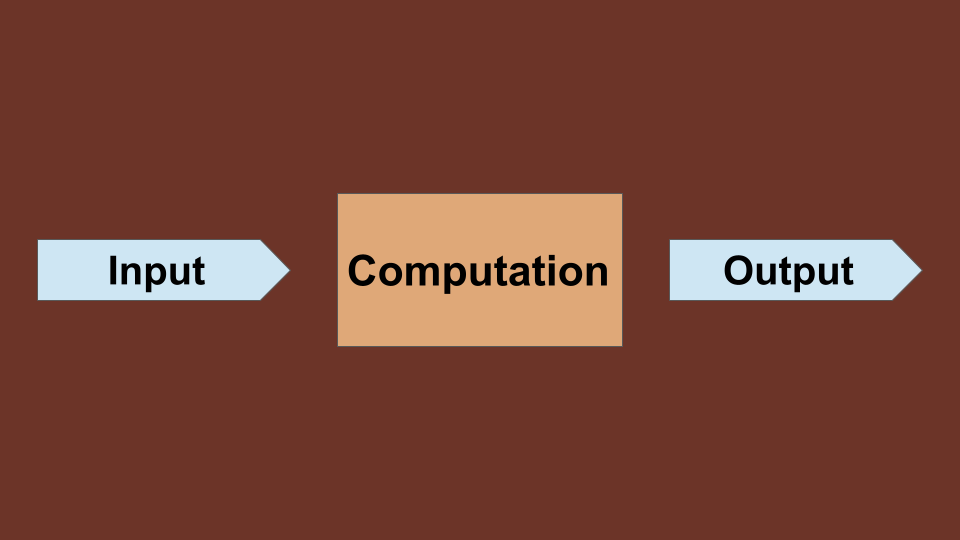
\includegraphics[width=0.8\textwidth]{standard computation model.png}
	\caption{یک واحد محاسباتی که مقادیری را به عنوان ورودی گرفته، پردازش کرده و سپس مقدار/مقادیر خروجی را ارائه کرده است.}
\end{figure}


در تصویر بالا یک نمود ساده از کامپیوتر‌های امروزی ارائه شده است. در دنیای واقعی مقدار ورودی می‌تواند از هر منبعی‌ تأمین شده باشد. با این وجود هدف ما بررسی منابع تولید ورودی نیست؛‌ بلکه هدف بررسی مقادیر ورودی (به صورت ایزوله) می‌باشد. می‌توان درنظر گرفت که ورودی داده شده و خروجی نهایی،‌هر دو در قالب یک رشته از اعداد باینری، ماتریس و یا هرقالب مدنظر کاربر باشند.

مهم‌ترین نکته درباره‌ی این واحد محاسباتی،‌ \textbf{در دسترس بودن کل مقادیر ورودی برای واحد پردازش} است. به عبارت دیگر\textbf{ واحد پردازش می‌تواند تمامی مقادیر ورودی را دریافت کرده و تشخیص} دهد. 

\section{مدل کوئری}
در مدل کوئری، داده‌های ورودی توسط یک تابع تولید می‌شوند. واحد محاسباتی دسترسی به تابع تولیدورودی دارد و می‌تواند برای دریافت داده‌های جدید،‌از تابع یاد شده،‌درخواست کند.

\begin{figure}[ht]
	\centering
	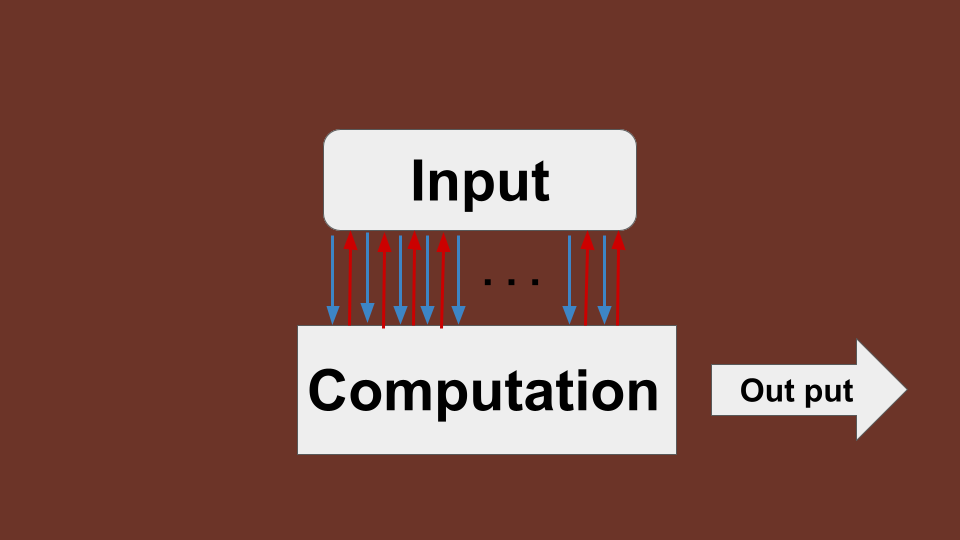
\includegraphics[width=0.8\textwidth]{Query computation model.png}
	\caption{شکل بالا نمود مدل محاسباتی‌کوئری است. واحد محاسباتی برای دریافت داده‌های جدید نیاز به درخواست از تابع \lr{input} دارد. خطوط قرمز و روبه‌بالا نشان از درخواست واحد محاسباتی و خطوط آبی روبه‌پایین نشان از پاسخ واحد \lr{input}می‌باشد.}
\end{figure}


در این مدل واحد محاسباتی دیگر داده‌ها را در قالب رشته‌ای از اطلاعات دردسترس ندارد؛ بلکه می‌تواند آن‌ها را از بخش \lr{input} دریافت کند. در گاهی از مواقع به سیستم \lr{input}،‌\lr{oracle} یا جعبه‌ی سیاه می‌گویند. تابع \lr{Oracle } یا جعبه‌ی سیاه یک سیستم است که ما به عنوان ناظر به سازوکار داخلی آن و  تمامی اطلاعات آن دسترسی نداریم و فقط می‌توانیم مقادیر مجاز را به آن داده و مقادیر خروجی را دریافت کنیم. 

تابع \lr{oracle} به صورت زیر تعریف می‌شود:
\begin{center}
$$
\left\{
\begin{array}{ll}
f : \sum^n = \sum^m\\
Which : m, n \in \mathbb{N}
\end{array}
\right.
$$
\end{center}

ما در این نظریه کوئری‌ها را می‌شماریم و وضعیت آن‌‌ها را بررسی می‌کنیم.

\section{معرفی و پیاده سازی الگوریتم دوچ}

\subsection{مسئله‌ی دوچ}
الگوریتم \lr{Deutsch} اولین و ساده‌ترین الگوریتم کوانتومی‌ است. این الگوریتم برای اولین بار در سال 1985 در مقاله‌ای مطرح شد؛ که توسط دیوید دوچ\footnote{David Deutsch} نوشته شده‌‌بود. این الگوریتم نقطه‌ی شروعی برای اثبات برتری کامپیوترهای کوانتومی نسبت به کامپوترهای کلاسیک است.

مسئله‌ی \lr{Deutsch} یکی از ساده‌ترین مفاهیم ممکن را مطرح می‌کند. اگر یک تابع به فرم زیر تعریف شود: 
\begin{center}
	$f : \sum \rightarrow \sum$
\end{center}
هدف بررسی ثابت بودن یا متعادل\footnote{Constante or balanse.} بودن تابع \lr{f} است. 
به‌طور کلی، درساده‌ترین حالت، می‌توان چهار وضعیت را برای تابع $f : \sum \rightarrow \sum$ درنظر گرفت:\\
\begin{figure}[ht]
	\centering
	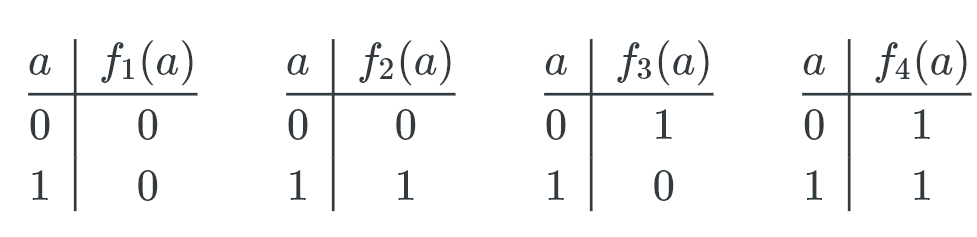
\includegraphics[width=0.8\textwidth]{Constantorbalanse.png}
	\caption{}
\end{figure}\\
در شکل بالا توابع \lr{f 1} , \lr{f 4} توابع ثابت و توابع \lr{f 2} و \lr{f 3} توابع متعادل هستند.
\begin{center}
\begin{tabular}{|c|c|}
	\hline
	\multicolumn{2}{|c|}{مسئله‌ی دوچ} \\
	\hline
	$f : \sum \rightarrow \sum$ & ورودی \\
	\hline
	صفر اگر تابع ثابت بود؛ یک اگر تابع متعادل بود.  & خروجی \\
	\hline
\end{tabular}
\end{center}
در الگوریتم‌های کلاسیک برای حل این مسئله، حداقل دو حالت باید بررسی شود.
\subsection{الگوریتم دوچ}
% quantum computer scinse : read it for yourself
% https://www.youtube.com/watch?v=2wticzHE1vs&t=2014s
% page 32

حال به بررسی الگوریتم دوچ می‌پردازیم. الگوریتمی که مسئله‌ی دوچ را با یک مدار کوانتومی حل می‌کند:\\
\begin{center}
\begin{figure}[ht]
	\centering
	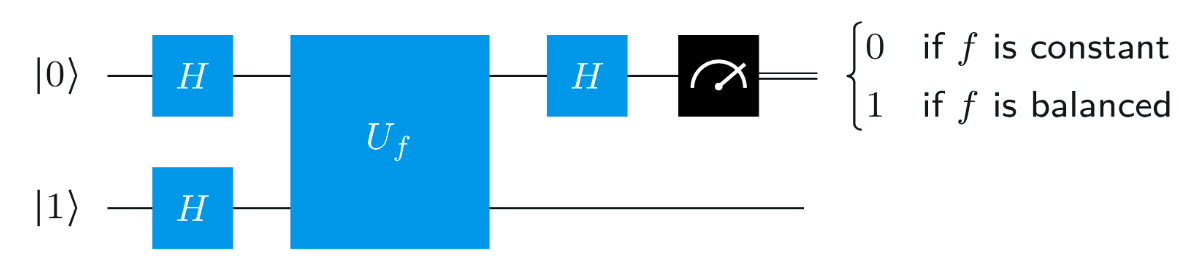
\includegraphics[width=0.8\textwidth]{Deutsch algorithm.png}
	\caption{}
\end{figure}
\end{center}

 
یک تغییر ساده در مدار شکل 1.3 نشان می دهد که چگونه مدارهای کوانتومی می توانند با پیاده سازی الگوریتم Deutsch از مدارهای کلاسیک پیشی بگیرند\footnote{ما در واقع یک نسخه ساده شده و بهبود یافته از الگوریتم اصلی را ارائه می دهیم.}. الگوریتم Deutsch ترکیبی از موازی سازی کوانتومی با خاصیتی از مکانیک کوانتوم به نام تداخل\footnote{how interference is using in deutsch algorithm : Interference is used in the Deutsch algorithm to distinguish between constant and balanced functions. A constant function is a function that always returns the same value, regardless of its input. A balanced function is a function that returns 0 for half of its inputs and 1 for the other half.
	
	The Deutsch algorithm works by first preparing two qubits in a superposition of states. The first qubit is prepared in the state |+⟩, which is the equal superposition of |0⟩ and |1⟩. The second qubit is prepared in the state |ψ⟩, which is a superposition of the states |0⟩ and |1⟩ with opposite phases.
	
	The two qubits are then passed through a quantum circuit that includes a Hadamard gate and a CNOT gate. The Hadamard gate transforms |+⟩ into the superposition |0⟩ + |1⟩, and the CNOT gate copies the state of the first qubit to the second qubit.
	
	After the quantum circuit has been executed, the two qubits are measured. If the first qubit is measured to be |0⟩, then the function f is constant. This is because the state |ψ⟩ is orthogonal to the state |0⟩, so the interference between the two states will destructively interfere.
	
	If the first qubit is measured to be |1⟩, then the function f is balanced. This is because the state |ψ⟩ is parallel to the state |1⟩, so the interference between the two states will constructively interfere.
	
	The Deutsch algorithm is a simple example of how quantum interference can be used to solve a problem that is difficult to solve classically. In this case, the Deutsch algorithm can distinguish between constant and balanced functions in a single step, while a classical computer would need to take an exponential number of steps.} است.
مشابه قبل،‌ابتدا از گیت هادامارد برای آماده سازی اولین کوبیت به عنوان superposition (|0〉 + |1〉)/√2 استفاده کنیم، اما اکنون کوبیت دوم y را با اعمال یک گیت هادامارد به حالت |1> به عنوان superposition (|0〉 - |1〉)/√2 آماده کنیم. به‌شکل زیر دقت کنید:



\begin{figure}[ht]
	\centering
	\includegraphics[width=0.8\textwidth]{Quantum circuit implementing Deutsch’s algorithm.png}
	\caption{پیاده‌سازی مدارکوانتومی‌ الگوریتم دوچ}
\end{figure}

\newpage

حالت ورودی:\\
\begin{center}
	$\vert\psi_{0}\rangle = \vert01\rangle$
\end{center}

سیستم دو کیوبیتی تشکیل شده،‌ پس از اعمال اثر دو گیت هادامارد می‌دهد:\\

\begin{center}
$\left|\psi_1\right\rangle=\left[\frac{|0\rangle+|1\rangle}{\sqrt{2}}\right]\left[\frac{|0\rangle-|1\rangle}{\sqrt{2}}\right]$
\end{center}
با کمی تأمل می‌توان دریافت که اگر Uf را به حالت |x〉(|0〉 - |1〉)/√2 اعمال کنیم، سپس به حالت (−1)f (x)|x〉(|0〉 - |1〉)/√2 می رسیم. بنابرین اعمال Uf به |ψ1〉 ما را با یکی از دو امکان زیر مواجه می کند:
\begin{center}
	$\left|\psi_2\right\rangle= \begin{cases} \pm\left[\frac{|0\rangle+|1\rangle}{\sqrt{2}}\right]\left[\frac{|0\rangle-|1\rangle}{\sqrt{2}}\right] & \text { if } f(0)=f(1) \\ \pm\left[\frac{|0\rangle-|1\rangle}{\sqrt{2}}\right]\left[\frac{|0\rangle-|1\rangle}{\sqrt{2}}\right] & \text { if } f(0) \neq f(1) \end{cases}$
\end{center}
با اعمال آخرین گیت هادامارد روی کیوبیت اول به حالت زیر خواهیم رسید:
\begin{center}
	$\left|\psi_3\right\rangle= \begin{cases} \pm|0\rangle\left[\frac{|0\rangle-|1\rangle}{\sqrt{2}}\right] & \text { if } f(0)=f(1) \\ \pm|1\rangle\left[\frac{|0\rangle-|1\rangle}{\sqrt{2}}\right] & \text { if } f(0) \neq f(1) \end{cases}$
\end{center}
با درنظر گرفتن شرایط زیر می‌توان $\vert\psi_{3}\rangle$ را به شکل زیر بازنویسی کرد:

$$
\begin{aligned}
	\left\{
	\begin{aligned}
		f(0) &= f(1) 
		\implies \qquad f(0) \oplus f(1) &= 0\\
		f(0) &\neq f(1) 
		\implies \qquad f(0) \oplus f(1) &= 1
	\end{aligned}
	\right.
\end{aligned}$$

از این رو:

\begin{center}
	$\left|\psi_3\right\rangle= \pm|f(0) \oplus f(1)\rangle\left[\frac{|0\rangle-|1\rangle}{\sqrt{2}}\right]$
\end{center}
بنابراین با اندازه گیری کیوبیت اول می توانیم $f(0) \oplus f(1)$ را تعیین کنیم. واقعاً جالب است! مدار کوانتومی به ما توانایی تعیین یک ویژگی جهانی از $f(x)$، یعنی$ f(0)\oplus f(1)$ را داده است، با استفاده از تنها یک ارزیابی از $f(x)$!این سریعتر از آن چیزی است که با یک دستگاه کلاسیک امکان‌پذیر است،یک دستگاه کلاسیک حداقل به دو ارزیابی نیاز دارد.
این مثال تفاوت بین موازی‌سازی کوانتومی و الگوریتم‌های تصادفی کلاسیک را برجسته می‌کند. به سادگی، ممکن است تصور شود که حالت $\vert0\rangle \vert f(0) \rangle + \vert1\rangle \vert f(1) \rangle$ مطابقت نزدیکی با یک رایانه کلاسیک تصادفی دارد که هرکدام از حالات $ f (0)$ یا$ f (1) $ با احتمال $1/2$ اندازه‌گیری می‌کند.
تفاوت این است که در یک رایانه کلاسیک این دو گزینه همیشه یکدیگر را حذف می‌کنند. در یک رایانه کوانتومی، امکان دارد که دو گزینه با یکدیگر تداخل داشته باشند تا برخی از خواص کلی تابع $f$ را با استفاده از چیزی شبیه به گیت هادامارد برای بازترکیب گزینه‌های مختلف، مانند آنچه در الگوریتم دوچ انجام شد، به دست آورند.
اساس طراحی بسیاری از الگوریتم‌های کوانتومی این است که یک انتخاب هوشمندانه از تابع و تبدیل نهایی اجازه می‌دهد تا اطلاعات جهانی مفیدی در مورد تابع تعیین شود - اطلاعاتی که نمی‌توان به سرعت در یک رایانه کلاسیک به دست آورد.

\section{الگوریتم دوچ - جوزا}
Deutsch’s algorithm is a simple case of a more general quantum algorithm, which we shall
refer to as the Deutsch–Jozsa algorithm. The application, known as Deutsch’s problem,
may be described as the following game. Alice, in Amsterdam, selects a number x from
0 to 2n − 1, and mails it in a letter to Bob, in Boston. Bob calculates some function
f (x) and replies with the result, which is either 0 or 1. Now, Bob has promised to use
a function f which is of one of two kinds; either f (x) is constant for all values of x,
or else f (x) is balanced, that is, equal to 1 for exactly half of all the possible x, and 0
for the other half. Alice’s goal is to determine with certainty whether Bob has chosen a
constant or a balanced function, corresponding with him as little as possible. How fast
can she succeed?

الگوریتم دوچ توضیح ساده از یک الگوریتم کوانتومی عمومی‌تر است که به عنوان الگوریتم دوچ-جوزا شناخته می‌شود. کاربرد این الگوریتم، که به عنوان مشکل دوچ شناخته می‌شود، به شرح زیر است:

آلیس، در آمستردام، یک عدد x را از بازه‌ $[0, 2^n-1]$ انتخاب می‌کند و آن را در یک نامه به باب، در بوستون، می‌فرستد. باب یک تابع$ f(x)$ را محاسبه می‌کند و نتیجه را که 0 یا 1 است، ارسال می‌کند. اکنون، باب قول داده است که از یک مدل تابع استفاده خواهد کرد؛ این تابع یا$ f(x)$ که برای همه مقادیر $x$ ثابت است، یا $f(x)$ متعادل است، یعنی‌ حاصل آن برای دقیقاً نیمی از همه xهای ممکن برابر با 1 است و برای نیمی دیگر برابر با 0 است.

هدف آلیس این است که با اطمینان و بکار بستن کمترین گام‌های ممکن تعیین کند که باب یک تابع ثابت یا متعادل را انتخاب کرده است. او چگونه می‌تواند به سرعت موفق شود؟

در حالت کلاسیک، آلیس ممکن است فقط یک مقدار x را در هر نامه به باب ارسال کند. در بدترین حالت، الی باید حداقل $\frac{2^n}{2} + 1$ بار از باب سوال کند، زیرا ممکن است قبل از دریافت یک، $\frac{2^n}{2}$ مرتبه پاسخ $0$ را دریافت کند. آلیس باید یک را دریافت کند؛‌تا بتواند به او بگوید که تابع باب متعادل است. 

یعنی در بهترین الگوریتم کلاسیک که می تواند استفاده کند بنابراین به$\frac{2^n}{2} + 1$ پرسش نیاز دارد. توجه داشته باشید که در هر نامه، آلیس n بیت اطلاعات را به باب ارسال می کند. علاوه بر این، در این مثال، فاصله فیزیکی باب و آلیس و به تبع آن افزایش هزینه محاسبه $f(x)$ و دشواری‌های احتمالی اجرای تابع $f(x)$ درنظر گرفته نشده‌است.

	اگر باب و آلیس بتوانند کوبیت ها را به جای بیت های کلاسیک مبادله کنند، و اگر باب موافقت کند $f (x)$ را با استفاده از تبدیل یکه‌ی \lr{$U_{f}$} محاسبه کند، سپس آلیس می تواند هدف خود را در یک مکاتبه با باب و با استفاده از الگوریتم زیر به دست آورد.
	
	با توجه به الگوریتم دوچ، آلیس یک رجیستر n کوبیتی را برای ذخیره پرس و جو خود آماده می کند و یک رجیستر کوبیت واحد را که به باب می دهد تا پاسخ را در آن ذخیره کند. او هر دو رجیستر پرس و جو و پاسخ خود را در یک حالت برهمنهی آماده می کند. باب f(x) را با استفاده از موازی سازی کوانتومی ارزیابی می کند و نتیجه را به آلیس برمی گرداند. آلیس سپس با استفاده از اعمال تبدیل هادامارد روی رجیستر پرس و جو(n-کیوبیتی)، حالات برهمنهی تداخل می‌دهد و با انجام یک اندازه گیری مناسب، تعیین می کند که آیا f ثابت یا متعادل است.
		
	گام‌های خاص الگوریتم در شکل 1.20 نشان داده شده است. بیایید با دنبال کردن این مدار، به بررسی حالات ایجاد شده بپردازیم.
	حالت ورودی |ψ0〉 = |0〉⊗n|1〉 (1.46)؛‌ شبیه حالت معادله (1.41) است، اما در اینجا رجیستر پرس و جو وضعیت n کوبیت را توصیف می‌کند که همه در حالت |0〉 آماده شده‌اند. پس از اعمال تبدیل هامادارد روی رجیستر پرس و جو  و روی رجیستر پاسخ، می‌توان نوشت:
	
	|ψ1〉 = ∑x∈{0,1}n|x〉√2n[ |0〉 − |1〉√2]
	
	
	
	The query register is now a superposition of all values, and the answer register is in an evenly weighted superposition of 0 and 1. Next, the function f is evaluated (by Bob)
	using Uf : |x, y〉 → |x, y ⊕ f (x)〉, giving (1.48) Alice now has a set of qubits in which the result of Bob’s function evaluation is stored
	in the amplitude of the qubit superposition state. She now interferes terms in the super-
	position using a Hadamard transform on the query register. To determine the result of
	the Hadamard transform it helps to first calculate the effect of the Hadamard transform
	on a state |x〉. By checking the cases x = 0 and x = 1 separately we see that for a single
	qubit H|x〉 = ∑
	z (−1)xz |z〉/√2. Thus (1.49) This can be summarized more succinctly in the very useful equation(1.50) where x · z is the bitwise inner product of x and z, modulo 2. Using this equation
	and (1.48) we can now evaluate |ψ3〉,(1.51) Alice now observes the query register. Note that the amplitude for the state |0〉⊗n is
	∑
	x(−1)f (x)/2n. 
	
	
	رجیستر پرس و جو اکنون یک برهمنهی از همه مقادیر ممکن به‌شمار می‌آید؛ درحالی که رجیستر پاسخ در یک برهمنهی به طور مساوی وزن شده از 0 و 1 محسوب می‌شود\footnote{یعنی احتمال رخ‌دادن صفر و یک یکسان است.}.
	
در مرحله بعد، تابع f توسط باب و به شکل Uf : |x, y〉 → |x, y ⊕ (x)〉f  ارزیابی می شود ، که (1.48) را می دهد.
	
	آلیس اکنون یک مجموعه کوبیت دارد که در آن نتیجه اعمال تابع باب در دامنه کوبیت حالت برهمنهی ذخیره می شود. او اکنون با استفاده از تبدیل هادامارد روی رجیستر پرس و جو، عبارات را در حالت برهمنهی کوانتومی تداخل می کند.
	
	برای تعیین نتیجه تبدیل هادامارد، بهترست ابتدا اثر تبدیل هادامارد را روی یک حالت |x〉 محاسبه کنیم. با بررسی موارد x = 0 و x = 1 به صورت جداگانه می بینیم که برای یک کوبیت واحد H|x〉 = ∑z (−1)xz |z〉/√2 می‌باشد. بنابراین (1.49)
	
	این را می توان به طور خلاصه در معادله بسیار مفید زیر خلاصه کرد:
	
	(1.50)
	
	جایی که x · z bitwise inner product x و z است، به modulo 2.
	
	با استفاده از این معادله و (1.48) اکنون می توانیم |ψ3〉 را ارزیابی کنیم:
	
	(1.51)
	
	آلیس اکنون رجیستر پرس و جو را مشاهده می کند. توجه داشته باشید که دامنه برای حالت |0〉⊗n است
	∑
	x(−1)f (x)/2n.
	
	
	
	
	
	\textbf{از استاد بپرس اشکاااااللللل}
	
	Let’s look at the two possible cases – f constant and f balanced – to
	discern what happens. In the case where f is constant the amplitude for |0〉⊗n is +1 or
	−1, depending on the constant value f (x) takes. Because |ψ3〉 is of unit length it follows
	that all the other amplitudes must be zero, and an observation will yield 0s for all qubits
	in the query register. If f is balanced then the positive and negative contributions to the
	amplitude for |0〉⊗n cancel, leaving an amplitude of zero, and a measurement must yield
	a result other than 0 on at least one qubit in the query register. Summarizing, if Alice measures all 0s then the function is constant; otherwise the function is balanced. The
	Deutsch–Jozsa algorithm is summarized below.
	
	
	بیایید به دو مورد ممکن - f ثابت و f متعادل - نگاه کنیم تا ببینیم چه اتفاقی می افتد.
	
	در صورتی که f ثابت باشد، دامنه برای حالت |0〉⊗n برابر است با +1 یا −1، بسته به مقدار ثابت f (x) که می‌گیرد.
	
	از آنجایی که |ψ3〉 طول واحد است، نتیجه می‌گیریم که تمام دامنه‌های دیگر باید صفر باشند، و یک مشاهده 0 را برای همه کوبیت‌ها در رجیستر پرس و جو به همراه خواهد داشت.
	
	اگر f متعادل باشد، سهم مثبت و منفی دامنه برای |0〉⊗n خنثی می‌شود، و یک دامنه صفر باقی می‌ماند، و یک اندازه‌گیری باید نتیجه‌ای غیر از 0 را در حداقل یک کوبیت در رجیستر پرس و جو به همراه داشته باشد.
	
	به طور خلاصه، اگر الی همه 0 را اندازه گیری کند، تابع ثابت است؛ در غیر این صورت تابع متعادل است.
	
	الگوریتم Deutsch-Jozsa در زیر خلاصه شده است:
	
	
	
	
	
	Algorithm: Deutsch–Jozsa
	Inputs: (1) A black box Uf which performs the transformation
	|x〉|y〉 → |x〉|y ⊕ f (x)〉, for x ∈ {0, . . . , 2n − 1} and f (x) ∈ {0, 1}. It is
	promised that f (x) is either constant for all values of x, or else f (x) is balanced,
	that is, equal to 1 for exactly half of all the possible x, and 0 for the other half.
	Outputs: 0 if and only if f is constant.
	Runtime: One evaluation of Uf . Always succeeds.
	Procedure:
	1. |0〉⊗n|1〉 initialize state
	2. → 1
	√2n
	2n −1∑
	x=0
	|x〉
	[ |0〉 − |1〉
	√2
	] create superposition using
	Hadamard gates
	3. → ∑
	x
	(−1)f (x)|x〉
	[ |0〉 − |1〉
	√2
	]
	calculate function f using Uf
	4. → ∑
	z
	∑
	x
	(−1)x·z+f (x)|z〉
	√2n
	[ |0〉 − |1〉
	√2
	]
	perform Hadamard transform
	5. → z measure to obtain final output z
	We’ve shown that a quantum computer can solve Deutsch’s problem with one evalu-
	ation of the function f compared to the classical requirement for 2n/2 + 1 evaluations.
	This appears impressive, but there are several important caveats. First, Deutsch’s prob-
	lem is not an especially important problem; it has no known applications. Second, the
	comparison between classical and quantum algorithms is in some ways an apples and
	oranges comparison, as the method for evaluating the function is quite different in the
	two cases. Third, if Alice is allowed to use a probabilistic classical computer, then by
	asking Bob to evaluate f (x) for a few randomly chosen x she can very quickly determine
	with high probability whether f is constant or balanced. This probabilistic scenario is
	perhaps more realistic than the deterministic scenario we have been considering. Despite
	these caveats, the Deutsch–Jozsa algorithm contains the seeds for more impressive quan-
	tum algorithms, and it is enlightening to attempt to understand the principles behind its
	operation.
	الگوریتم: Deutsch–Jozsa
	ورودی‌ها: (1) یک جعبه سیاه Uf که تبدیل زیر را انجام می‌دهد
	|x〉|y〉 → |x〉|y ⊕ f (x)〉, برای x ∈ {0، ...، 2n - 1} و f (x) ∈ {0، 1}. قول داده شده است که f (x) برای همه مقادیر x ثابت است یا f (x) متعادل است،
	یعنی برای دقیقاً نیمی از همه xهای ممکن برابر با 1 و برای نیمی دیگر 0 است.
	خروجی: 0 اگر و فقط اگر f ثابت باشد.
	زمان اجرا: یک ارزیابی Uf. همیشه موفق می شود.
	روش:
	
	|0〉⊗n|1〉 حالت را initialize کنید
	→ 1 √2n 2n −1∑ x=0 |x〉 [ |0〉 − |1〉 √2 ] ایجاد superposition با استفاده از دروازه‌های Hadamard
	→ ∑ x (−1)f (x)|x〉 [ |0〉 − |1〉 √2 ] تابع f را با استفاده از Uf محاسبه کنید
	→ ∑ z ∑ x (−1)x·z+f (x)|z〉 √2n [ |0〉 − |1〉 √2 ] تبدیل Hadamard را انجام دهید
	→ z اندازه گیری کنید تا خروجی نهایی z را بدست آورید ما نشان داده‌ایم که یک کامپیوتر کوانتومی می‌تواند مشکل Deutsch را با یک ارزیابی حل کند – ارزشیابی تابع f در مقایسه با نیاز کلاسیک برای 2n/2 + 1 ارزیابی. این به نظر چشمگیر است، اما چند نکته مهم وجود دارد. اول، مشکل Deutsch نیست یک مشکل مهم است؛ هیچ کاربرد شناخته شده ای ندارد. دوم، مقایسه بین الگوریتم های کلاسیک و کوانتومی تا حدودی مقایسه سیب و پرتقال است، زیرا روش برای ارزیابی تابع در دو مورد بسیار متفاوت است. سوم، اگر آلیس مجاز باشد از یک کامپیوتر کلاسیک احتمالی استفاده کند، سپس با درخواست از باب برای ارزیابی f (x) برای چند x به صورت تصادفی می تواند بسیار سریع تعیین کند با احتمال بالا اینکه f ثابت یا متعادل است. این سناریو احتمالی است شاید واقع بینانه تر از سناریوی determinstic که ما در نظر گرفته ایم. علیرغم این ظرافت ها، الگوریتم Deutsch–Jozsa حاوی بذرهای الگوریتم های کوانتومی بیشتر و چشمگیرتر است، و درک اصول پشت آن روشنگر است. عملکرد آن.
	
	
	
\section{ساخت یک اوراکل کوانتومی}
بیایید راه های مختلفی را ببینیم که می توانیم یک اوراکل کوانتومی ایجاد کنیم.

برای یک تابع ثابت، ساده است:

اگر f(x) = 0، گیت را به کیوبیت در ثبات 2 اعمال کنید.
اگر f(x) = 1، گیت را به کیوبیت در ثبات 2 اعمال کنید.

برای عملکرد متعادل، مدارهای مختلفی وجود دارد که می توانیم ایجاد کنیم. یکی از راه‌هایی که می‌توانیم متوازن بودن مدار خود را تضمین کنیم، انجام یک CNOT برای هر کیوبیت در ثبات 1، با کیوبیت موجود در ثبات 2 به عنوان هدف است. مثلا:

\begin{center}
	\begin{figure}[ht]
		\centering
		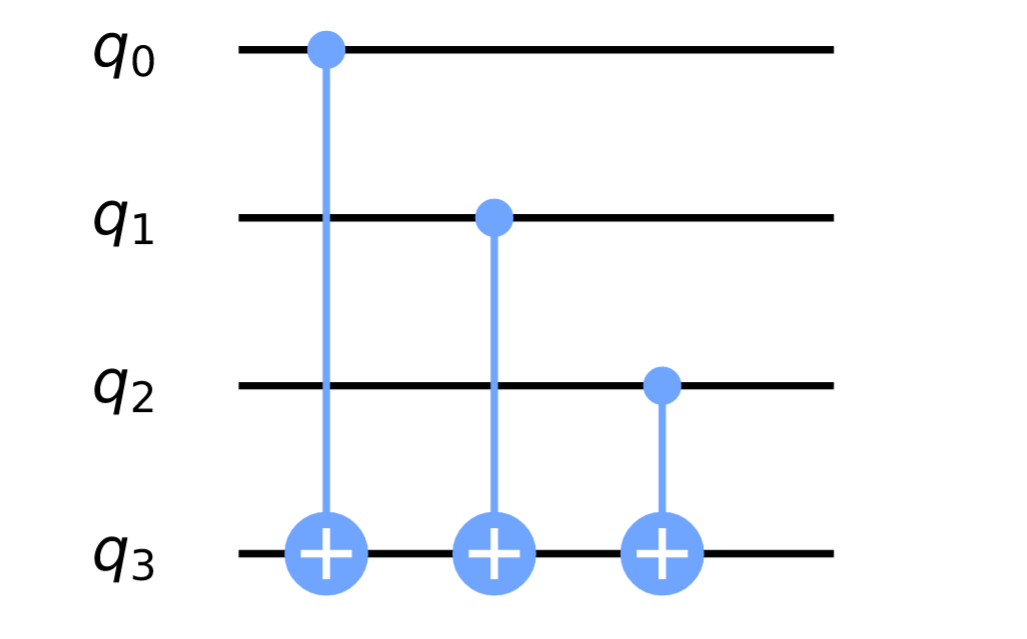
\includegraphics[width=0.8\textwidth]{oraclecon.png}
		\caption{}
	\end{figure}
\end{center}




در تصویر بالا، سه کیوبیت بالا، رجیستر ورودی را تشکیل می دهند و کیوبیت پایین، ثبات خروجی است. در جدول زیر می‌توانیم ببینیم کدام حالت‌های ورودی کدام خروجی را می‌دهند:
\begin{table}[h]
	\centering
	\begin{tabular}{|c|c|}
		\hline
		حالاتی ورودی که به خروجی صفر منجر می‌شوند &  حالاتی ورودی که به خروجی صفر منجر می‌شوند \\ \hline
		000 & 001 \\ \hline
		011 & 100 \\ \hline
		101 & 010 \\ \hline
		110 & 111 \\ \hline
	\end{tabular}
	\caption{This is a simple table.}
\end{table}
ما می توانیم نتایج را تغییر دهیم و در عین حال تعادل آنها را با قرار دادن کنترل های انتخاب شده در X-Gates حفظ کنیم. برای مثال، مدار و جدول نتایج آن را در زیر ببینید:
\begin{center}
	\begin{figure}[ht]
		\centering
		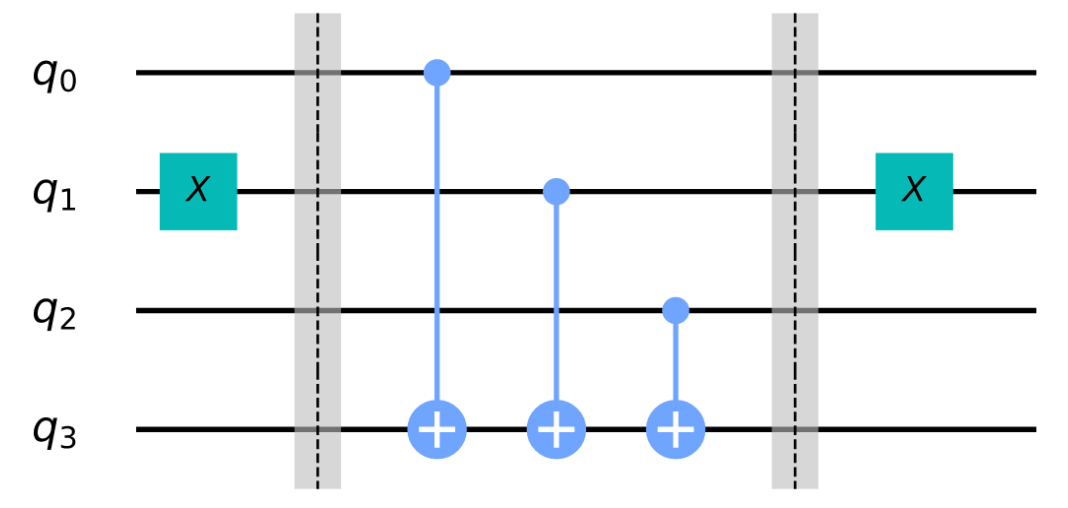
\includegraphics[width=0.8\textwidth]{oraclebalance.png}
		\caption{}
	\end{figure}
\end{center}


\begin{table}[h]
	\centering
	\begin{tabular}{|c|c|}
		\hline
		حالاتی ورودی که به خروجی صفر منجر می‌شوند &  حالاتی ورودی که به خروجی صفر منجر می‌شوند \\ \hline
		001 & 000 \\ \hline
		010 & 011 \\ \hline
		100 & 101 \\ \hline
		111 & 110 \\ \hline
	\end{tabular}
	\caption{This is a simple table.}
\end{table}



% implimentation : https://learn.qiskit.org/course/ch-algorithms/deutsch-jozsa-algorithm

\chapter{شبیه‌سازی پدیده‌های کوانتومی}
در این بخش قصد داریم به بررسی پروتکل‌های ابتدایی در نظریه‌ی اطلاعات کوانتومی بپردازیم. تمامی این پروتکل‌ها به تعداد کمی کیوبیت نیاز دارند؛ و در آزمایشگاه به صورت تجربی پیاده‌سازی شده‌اند. 
\section{Bell states}
% https://www.youtube.com/watch?v=I0jH1_H3x1o
% pls search about bell eq
در اغلب موارد، سیستم از دو کیوبیت درهمتنیده تشکیل شده‌است. تابع حالت این سیستم‌ها به شکل زیر تعریف می‌شوند:
\begin{center}
	$\vert \psi_{00} \rangle = \frac{1}{\sqrt{2}}(|00\rangle + |11\rangle)$
\end{center}
برای آماده‌سازی این حالت کوانتومی‌، در حالت \lr{$\vert0\rangle$} داریم. با اعمال یک گیت هدامارد روی یکی از کیوبیت‌ها و سپس با کنترل‌ آن با گیت \lr{CNOT}، (به نحوی که کیوبیت دوم هدف قرارگیرد.) می‌توان به یک حالت درهمتنیده رسید. می‌توان این مراحل را به شکل زیر شرح داد:
\begin{center}
	$\vert\psi_{00}\rangle = C_{10}H_{1}\vert00\rangle$
\end{center}

%می‌توان رابطه‌ی بالا را به هریک از حالات $\vert00\rangle, \vert 01\rangl, \vert 10\rangl, \vert 11\rangl$ تعمیم داد:%
\[
\vert\psi_{xy}\rangle = C_{10}H_{1}\vert xy \rangle
\]

از آنجایی که چهار حالت $\vert xy\rangle$ یک مجموعه متعامد هستند و گیت‌های هادامارد و cNOT یکه هستند، چهار حالت درهم تنیده $\vert \psi_{xy}\rangle$ نیز یک مجموعه متعامد هستند، که به نام پایه Bell نامگذاری شده‌اند.  می‌توان رابطه‌ی بالا را یک حالت کلی تعمیم داد:

% read about bell state equation
\begin{center}
$\vert \psi_{xy}\rangle = C10H1X^{x}_{1} X^{y}_{0} \vert00\rangle$\\
\end{center}

\begin{figure}
	\centering
	\begin{subfigure}[b]{}
		\centering
		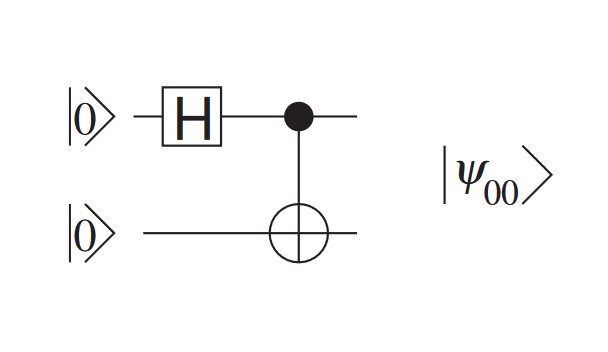
\includegraphics[width=0.2\textwidth]{psi00.png}
		\caption{$y=x$}
		\label{fig:y equals x}
	\end{subfigure}
	\hfill
	\begin{subfigure}[b]{}
		\centering
		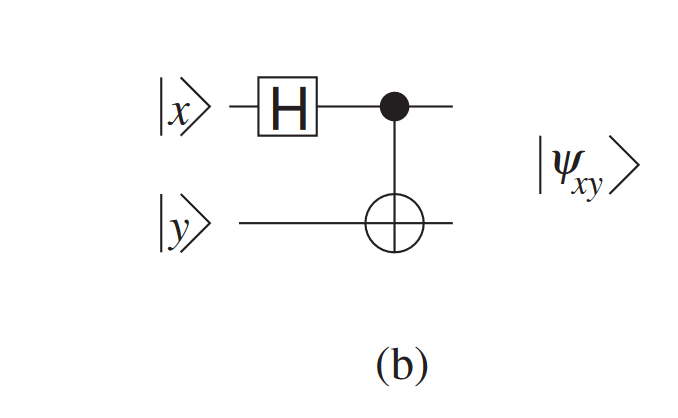
\includegraphics[width=0.2\textwidth]{psixy.png}
		\caption{$y=3\sin x$}
		\label{fig:three sin x}
	\end{subfigure}
	\caption{(a) A circuit that creates the entangled state
		|ψ00〉 = 1√2
		(|00〉 + |11〉) from the unentangled computational-basis
		state |00〉. (b) A circuit that creates the four orthonormal entangled
		Bell states |ψxy〉 from the unentangled computational-basis state |xy〉}
	\label{fig:three graphs}
\end{figure}


درنظر داشته باشید که حالات بل قابل تبدیل به یکدیگرند؛ با کمک رابطه‌ی تعمیم یافته ‌می‌توان از هر حالت بل به حالت $\vert00 \rangle$ رسید.
توضیحات درباره‌ی تبدیلات بنویس

این روابط به شکل‌های متعدد قابل بیان است که از حوصله‌ی بحث خارج است.
\newpage






\section{entanglement}
\newpage



\section{رمزگذاری متراکم کوانتومی}
% from quantum computation l chuang

رمزگذاری متراکم کوانتومی\footnote{\lr{Quantum super dense coding}} یک کاربرد ساده اما شگفت‌انگیز از مفاهیم ابتدایی مکانیک کوانتومی است. این کاربرد، همه ایده‌های اساسی و ابتدایی مکانیک کوانتومی را به روشی ملموس و غیرقابل‌توضیح ترکیب می‌کند، بنابراین مثالی ایده‌آل از اهداف و وظایف پردازش اطلاعات است که می‌توان با استفاده از مکانیک کوانتومی انجام داد.

رمزگذاری متراکم شامل دو طرفین است که به طور معمول به عنوان «آلیس» و «باب» شناخته می‌شوند، که از هم فاصله زیادی دارند. هدف آنها انتقال برخی اطلاعات کلاسیک از آلیس به باب است. فرض کنید آلیس قصد دارد دوبیت داده‌ی کلاسیک را برای باب ارسال کند، اما فقط مجاز است یک کوبیت به باب ارسال کند. آیا می‌تواند به هدف خود برسد؟

رمزگذاری متراکم به ما می‌گوید که پاسخ این سؤال بله است. فرض کنید آلیس و باب در ابتدا یک جفت کوبیت در حالت درهم‌تنیده زیر به اشتراک می‌گذارند:

|ψ〉 = |00〉 + |11〉
√2 . (2.133)\\
=========

بیانات چی بیتی
آلیس می‌تواند با استفاده از این جفت کوبیت‌های درهم‌تنیده، دو بیت کلاسیک را به باب منتقل کند. او این کار را با اعمال یک تبدیل واحد به کوبیت خود انجام می‌دهد، بسته به اینکه می‌خواهد کدام دو بیت کلاسیک را به باب ارسال کند. به عنوان مثال، اگر آلیس می‌خواهد بیت‌های 00 را به باب ارسال کند، او تبدیل 1 را به کوبیت خود اعمال می‌کند.

این تبدیل واحد باعث می‌شود که کوبیت آلیس و کوبیت باب در یکی از چهار حالت بل اورتوگونال قرار گیرند. اگر آلیس کوبیت خود را در حالت |00〉 قرار دهد، کوبیت باب به طور خودکار به حالت |00〉 تبدیل می‌شود. این بدان معناست که آلیس دو بیت اطلاعات (0 و 0) را به باب منتقل کرده است.

باب سپس کوبیت خود را اندازه‌گیری می‌کند و مقدار 0 یا 1 را به دست می‌آورد. بسته به مقداری که باب اندازه‌گیری می‌کند، او می‌تواند دو بیت کلاسیک که آلیس به او ارسال کرده است را بازیابی کند.

رمزگذاری متراکم یک پروتکل کوانتومی بسیار کارآمد است که می‌تواند دو بیت کلاسیک را با ارسال یک کوبیت منتقل کند. این پروتکل می‌تواند در کاربردهای مختلفی مانند رمزنگاری کوانتومی و ارتباطات کوانتومی استفاده شود.\\
==========\\

همانطور که در شکل 2.3 قابل ملاحظه است؛ آلیس و باب، هرکدام یک کیوبیت در اختیار دارند. توجه داشته باشید که $\Psi$ یک حالت ثابت است؛ نیازی نیست که آلیس برای آماده‌سازی این حالت، کوبیتی را به باب ارسال کند. در عوض، ممکن است یک طرف ثالث قبلاً حالت درهم‌تنیده را آماده کند، یکی از کوبیت‌ها را به آلیس و دیگری را به باب ارسال کند.

با ارسال تک کوبیت آلیس  به باب، معلوم می‌شود که آلیس می‌تواند دو بیت اطلاعات کلاسیک را به باب منتقل کند. در اینجا روشی که او استفاده می‌کند؛ آورده شده است. اگر او بخواهد رشته‌بیت :

\begin{itemize}
	\item  $"00"$ را ارسال کند $\impliedby$ هیچ کاری روی کیوبیت خود انجام ندهد.
	\item $"01"$ را ارسال کند $\impliedby$ تبدیل دگرگونی فاز\footnote{phase flip} را روی کیوبیت خود اثر می‌دهد.
	\item  $"10"$ را ارسال کند $\impliedby$ گیت کوانتومی NOT، X، را به کوبیت خود اعمال می‌کند.
	\item  $"11"$ را ارسال کند $\impliedby$ تبدیل iY را به کوبیت خود اعمال می‌کند.
\end{itemize}
چهار حالت حاصل به راحتی قابل مشاهده هستند:\\
00 : |ψ〉 → |00〉 + |11〉
√2 (2.134)
01 : |ψ〉 → |00〉 − |11〉
√2 (2.135)
10 : |ψ〉 → |10〉 + |01〉
√2 (2.136)
11 : |ψ〉 → |01〉 − |10〉
√2 . (2.137)\\


همانطور که در بخش 1.3.6 اشاره کردیم، این چهار حالت به عنوان پایه بل، حالت‌های بل، یا جفت‌های EPR شناخته می‌شوند، به احترام چندین تن از پیشگامان که اولین بار از نوآوری درهم‌تنیدگی قدردانی کردند. توجه داشته باشید که حالت‌های بل یک پایه متعامد هستند، و بنابراین می‌توانند با اندازه‌گیری کوانتومی مناسب از یکدیگر متمایز شوند. اگر آلیس کوبیت خود را به باب بفرستد، و باب هر دو کوبیت را در اختیار داشته باشد، سپس با انجام اندازه‌گیری در پایه بل، باب می‌تواند تعیین کند که کدام یک از چهار رشته بیت ممکن را آلیس ارسال کرده است.

به طور خلاصه می‌توان گفت:
 آلیس، با تعامل و اثرگذاری تنها روی یک کوبیت، قادر به انتقال دو بیت اطلاعات به باب است. البته دو کوبیت در پروتکل دخیل هستند، اما آلیس هرگز نیازی به تعامل با کوبیت دوم ندارد. از نظر کلاسیک، وظیفه‌ای که آلیس انجام می‌دهد، اگر فقط یک بیت کلاسیک ارسال می‌کرد، غیرممکن بود.

علاوه بر این، پروتکل رمزگذاری متراکم، تا حدی در آزمایشگاه تأیید شده است.  یک نکته کلیدی را می‌توان در این مثال زیبا مشاهده کرد: اطلاعات فیزیکی است، و نظریه‌های فیزیکی شگفت‌انگیز مانند مکانیک کوانتوم ممکن است توانایی‌های پردازش اطلاعات شگفت‌انگیزی را پیش‌بینی کنند.



بیانات چی پی تی:
پروتکل سوپردنس کدینگ یک پروتکل کوانتومی است که آلیس می‌تواند از آن برای انتقال دو بیت کلاسیک به باب با ارسال یک کوبیت استفاده کند. پروتکل به شرح زیر است:

آلیس و باب یک جفت کوبیت درهم‌تنیده را با هم به اشتراک می‌گذارند.
آلیس می‌خواهد دو بیت کلاسیک، 00 یا 01 را به باب ارسال کند.
آلیس یک عمل واحد بر روی کوبیت خود اعمال می‌کند که بسته به بیت‌هایی که می‌خواهد به باب ارسال کند متفاوت است.
آلیس کوبیت خود را به باب می‌فرستد.
باب کوبیت را اندازه‌گیری می‌کند و دو بیت کلاسیکی که آلیس به او ارسال کرده است را دریافت می‌کند.
اگر آلیس یک عمل واحد بر روی کوبیت خود اعمال نکند، باب فقط می‌تواند یک بیت کلاسیک را دریافت کند. با این حال، اگر آلیس عمل واحد مناسب را اعمال کند، می‌تواند دو بیت کلاسیک را با ارسال یک کوبیت انتقال دهد.

پروتکل سوپردنس کدینگ یک مثال عالی از قدرت مکانیک کوانتوم در انتقال اطلاعات است. این پروتکل نشان می‌دهد که می‌توان با استفاده از قوانین مکانیک کوانتوم، اطلاعات را به روش‌های غیرممکن در فیزیک کلاسیک انتقال داد.
\newpage
\section{دوربری}
isac book
فرض کنید آلیس یک کیوبیت در حالت زیر دارد:
\begin{center}
$\vert \psi \rangle = \alpha\vert 0 \rangle + \beta\vert 1 \rangle $\\	
\end{center}

	کارول ممکن است با اعمال یک عملگر یکه‌ به یک کیوبیت در حالت استاندارد، کیوبیت را از حالت $\vert0\rangle$ به حالت $\vert\psi\rangle$  تبدیل کرده باشد. کارول بدون اعلام نوع عملگر یکه به آلیس،‌ کیوبیت را برای او ارسال می‌کند. 
	حال آلیس می‌خواهد بدون دسترسی داشتن به کیوبیت باب، تغییراتی را در کیوبیت او ایجاد کند؛ این تنها درصورتی ممکن است که کیوبیت باب و آلیس درهمتنیده باشند. هرچند آلیس و باب می‌توانند از طریق راه‌های کلاسیک(نظیر تلفنی صحبت کردن و ...) با یکدیگر ارتباط برقرار کنند؛ ولی نمی‌توانند دسترسی مستقیم به کیوبیت یکدیگر داشته باشند. 
	
	کیوبیت باب را می‌توان به حالت زیر تعریف کرد:
$\vert\phi\rangle = 1/\sqrt{2}(\vert0\rangle \vert0\rangle + \vert1\rangle\vert1\rangle)$ 
	
he no-cloning theorem prohibits duplicating the unknown state
of Alice’s first Qbit, either far away from her or nearby. But it turns
out to be possible for Alice and Bob to cooperate over the telephone
in assigning the state |ψ〉 to Bob’s member of the entangled pair. The
no-cloning theorem is not violated because in doing so Alice obliterates
all traces of the state |ψ〉 from either of her own Qbits. The process –
called teleporting the state from Alice to Bob – also eliminates the en-
tanglement Alice and Bob formerly shared. For each shared entangled
pair, they can teleport just a single 1-Qbit state. The term “teleporta-
tion” emphasizes that the state assignment acquired by Bob’s Qbit no
longer applies to Alice’s; it has been transported from her Qbit to his.
Here is how teleportation works. Alice’s first Qbit and the entangled
pair she shares with Bob are characterized by the 3-Qbit state
%|ψ〉a |〉ab = (α|0〉a + β|1〉a
) 1√2
(|0〉a |0〉b + |1〉a |1〉b
), (6.21)
where I have given the state symbols for the Qbits in Alice’s and Bob’s
possession subscripts a and b . To teleport the unknown state of her
Qbit to Bob’s member of the entangled pair, Alice first applies a cNOT
gate, using her first Qbit in the state |ψ〉 as the control and her member
of the shared entangled pair as the target. This produces the 3-Qbit
state
α|0〉a 1√2
(|0〉a |0〉b + |1〉a |1〉b
) + β|1〉a 1√2
(|1〉a |0〉b + |0〉a |1〉b
).
(6.22)
Next she applies a Hadamard transformation H to her first Qbit, giving
all three Qbits the state
α 1√2
(|0〉a + |1〉a
) 1√2
(|0〉a |0〉b + |1〉a |1〉b
)
+ β 1√2
(|0〉a − |1〉a
) 1√2
(|1〉a |0〉b + |0〉a |1〉b
)
= 1
2 |0〉a |0〉a
(α|0〉b + β|1〉b
) + 1
2 |1〉a |0〉a
(α|0〉b − β|1〉b
)
+ 1
2 |0〉a |1〉a
(α|1〉b + β|0〉b
) + 1
2 |1〉a |1〉a
(α|1〉b − β|0〉b
). (6.23)
Now Alice measures both Qbits in her possession. (As remarked
in Section 6.4, such an application of cNOT and Hadamard gates,
immediately followed by measurement gates, is called “measuring in
the Bell basis.”) If the result is 00, Bob’s Qbit will indeed acquire the
state |ψ〉 originally possessed by Alice’s first Qbit (whose state would
then be reduced to |0〉). But if the result of Alice’s measurement is 10,
01, or 11 then the state of Bob’s Qbit becomes
α|0〉b − β|1〉b , α|1〉b + β|0〉b , or α|1〉b − β|0〉b . (6.24)
In each of these three cases there is a unitary transformation that re-
stores the state of Bob’s Qbit to Alice’s original state |ψ〉. In the first
case we can apply Z (which leaves |0〉 alone but changes the sign of |1〉),
in the second case, X (which interchanges |0〉 and |1〉), and in the third
case, ZX.
6 . 5 TE L E P O R T A T I O N 151
So all Alice need do to transfer the state of her Qbit to Bob’s member
of their entangled pair is to telephone Bob and report to him the results
of her two measurements. He then knows whether the state has already
been transferred (if Alice’s result is 00) or what unitary transformation
he must apply to his member of the entangled pair in order to com-
plete the transfer (if Alice’s result is one of the other three.) Note the
resemblance to quantum error correction: by making a measurement
Alice acquires the information needed for Bob to reconstruct a partic-
ular quantum state, without anybody acquiring any information about
what the state actually is.
This appears to be remarkable. A general state of a Qbit is described
by two complex numbers α and β that take on a continuum of values,
constrained only by the requirement that |α|2 + |β|2 = 1. Yet, with the
aid of a standard entangled pair, whose state does not depend on α and
β, Alice is able to provide Bob with a Qbit described by the unknown
state, at the price of only two bits of classical information (giving the
results of her two measurements) and the loss of the entanglement of their pair.






But of course the teleportation process does not communicate to Bob the information that can be encoded in α and β. Bob is no more able to learn the values of α and β from manipulating his Qbit, now assigned the state |ψ〉, than Alice was able to do when it was her Qbit that was assigned the same state |ψ〉. On the other hand Alice’s state could be produced at a crucial stage of an elaborate quantum computation, and its transfer to Bob could enable him to continue with the computation on his own far-away quantum computer, s  one can achieve a nontrivial objective by such teleportations. Like dense coding, teleportation can also be constructed by manipulating an elementary classical circuit diagram, without going through any of the analysis in (6.21)–(6.24). Figure 6.5(a) shows a circuit that exchanges the state |ψ〉 = |x〉 of Alice’s Cbit with the state |0〉 of Bob’s Cbit, regardless of whether x = 0 or 1. The transfer is achieved by direct physical coupling between the two Cbits. As a linear quantum circuit it continues to perform this exchange for arbitrary superpositions, |ψ〉 = α|0〉 + β|1〉. The entire teleportation protocol can be constructed by appropriately expanding the two gates in Figure 6.5(a), with the aid of an ancillary Qbit. The aim of the expansion is to eliminate the direct interaction between Alice’s and Bob’s Qbits through the two cNOT gates in Figure 6.5(a), in favor of the telephoned message from Alice to Bob, and the interaction necessary to produce their shared pair of entangled Qbits (which can take place well before Alice has even acquired her Qbit in the state |ψ〉).





%In Figure 6.5(b) an ancillary Qbit, not acted upon throughout the process, is introduced in the state |φ〉 = H|0〉 = 1√2 (|0〉 + |1〉). (6.25) In Figure 6.5(c) the identities X = HZH and 1 = HH have been used to rewrite the cNOT gate on the right of Figure 6.5(b), and an additional cNOT gate has been added on the left, which acts as the identity, since X acts as the identity on the state H|0〉. Figure 6.5(d) follows from Figure 6.5(c) because the action of CZ is independent of which Qbit is the control and which the target, and because the two cNOT gates on the left of Figure 6.5(c) have exactly the same action as the three cNOT gates on the left of Figure 6.5(d): acting on the computational basis, both sets of gates apply X on both of the bottom two wires if the state of the top wire is |1〉 and act as the identity if the state of the top wire is |0〉. Figure 6.5(e) follows from Figure 6.5(d) if we write the |φ〉 on the left of Figure 6.5(d) as H|0〉 and explicitly write the |0〉 on the right of Figure 6.5(d) as H|φ〉. But Figure 6.5(e) is an automated version of teleportation. To relate it to ordinary teleportation, introduce mea- surements of the upper two Qbits after the circuit of Figure 6.5(e) has acted, as in Figure 6.5(f). Their effect is to collapse the states of each of the two upper wires randomly and independently to |0〉 or |1〉. But as noted in Section 3.6, measurement of a control Qbit commutes with any operation controlled by that Qbit, so the measurement gates can be moved to the positions they occupy in Figure 6.5(g). Figure 6.5(g) is precisely the teleportation protocol. The two gates on the left transform the two lower Qbits into the entangled state (6.20). The subsequent applications to the top two Qbits of cNOT followed by H followed by two measurement gates are precisely Alice’s “measurement in the Bell basis.” Since Alice knows the outcomes of the measurements, she knows whether the subsequent cNOT and CZ gates will or will not act, and she can replace these physical couplings by a phone call to Bob telling him whether or not to apply X and/or Z directly to his own Qbit. Figure 6.6 demonstrates that entanglement can also be teleported. The figure reproduces parts (b), (e), and (g) of Figure 6.5 with three changes. (1) A bar representing n Qbits in the n-Qbit state |〉i has been added above each part of the figure. No operations act on these additional Qbits. (2) The state to be teleported has been given a subscript i so it is now one of several possible states |ψi 〉. (3) Because of the linearity of the unitary gates we may sum over the index i . The effect of the circuit is to transfer participation in the entangled state ∑ i |i 〉|ψi 〉 from the third wire from the bottom to the bottom wire. So even if Alice’s Qbit has no state of its own but is entangled with other Qbits, Alice can use the same protocol to teleport its role in the entangled state over to Bob’s Qbit. The result is that Bob’s Qbit becomes entangled in exactly the same way Alice’s was, and Alice’s Qbit becomes entirely unentangled.
1
\newpage
how to determine a oracle\\
	
	
	
	
% https://learn.qiskit.org/course/ch-algorithms/quantum-circuits
	
	
	
\end{document}